\chapter{Árvores Binárias}
\chaplabel{binarytrees}

Este capítulo introduz uma das estruturas mais fundamentais na Ciência da Computação: árvores binárias. O uso da palavra \emph{árvore}
\index{árvore}%
\index{árvore!binária}%
\index{árvore!binária}%
vem do fato que, quando as desenhamos, o resultado frequentemente se assemelha às árvores de uma floresta. Existem muitas maneiras de definir uma árvore binária. Matematicamente, uma \emph{árvore binária} é um grafo conectado, não direcionado, finito, sem ciclos e sem nenhum vértice com grau maior que três.

Para muitas aplicações na ciência da computação, árvores binárias possuem \emph{raízes:}
\index{árvore!raiz}%
\index{árvore com raiz}%
um nó especial, #r#, com grau de no máximo dois é chamado de \emph{raiz} da árvore. Para cada nó $#u#\neq #r#$, o segundo nó no caminho de #u# para #r# é chamado de \emph{pai} de #u#.
\index{pai}%
cada um dos outros nós adjacentes a #u# é chamado de \emph{filho}
\index{filho} de #u#. Muitas da árvores binárias em que estamos interessados são \emph{ordenadas},
\index{árvore ordenada}%
\index{árvore!ordenada}%
assim distinguimos
entre o \emph{filho esquerdo} e o \emph{filho direito} de #u#.
\index{filho esquerdo}%
\index{filho!esquerdo}%
\index{filho direito}%
\index{filho!direito}%
 
Nas ilustrações, árvores binárias são comumente desenhadas da raiz para baixo, com a raiz no topo do desenho e os filhos esquerdo e direito dados respectivamente pelas posições esquerda e direita no desenho. 
(\figref{bintree-orientation}).  Por exemplo, a \figref{binary-tree}.a mostra uma árvore binária com nove nós.

\begin{figure}
  \begin{center}
    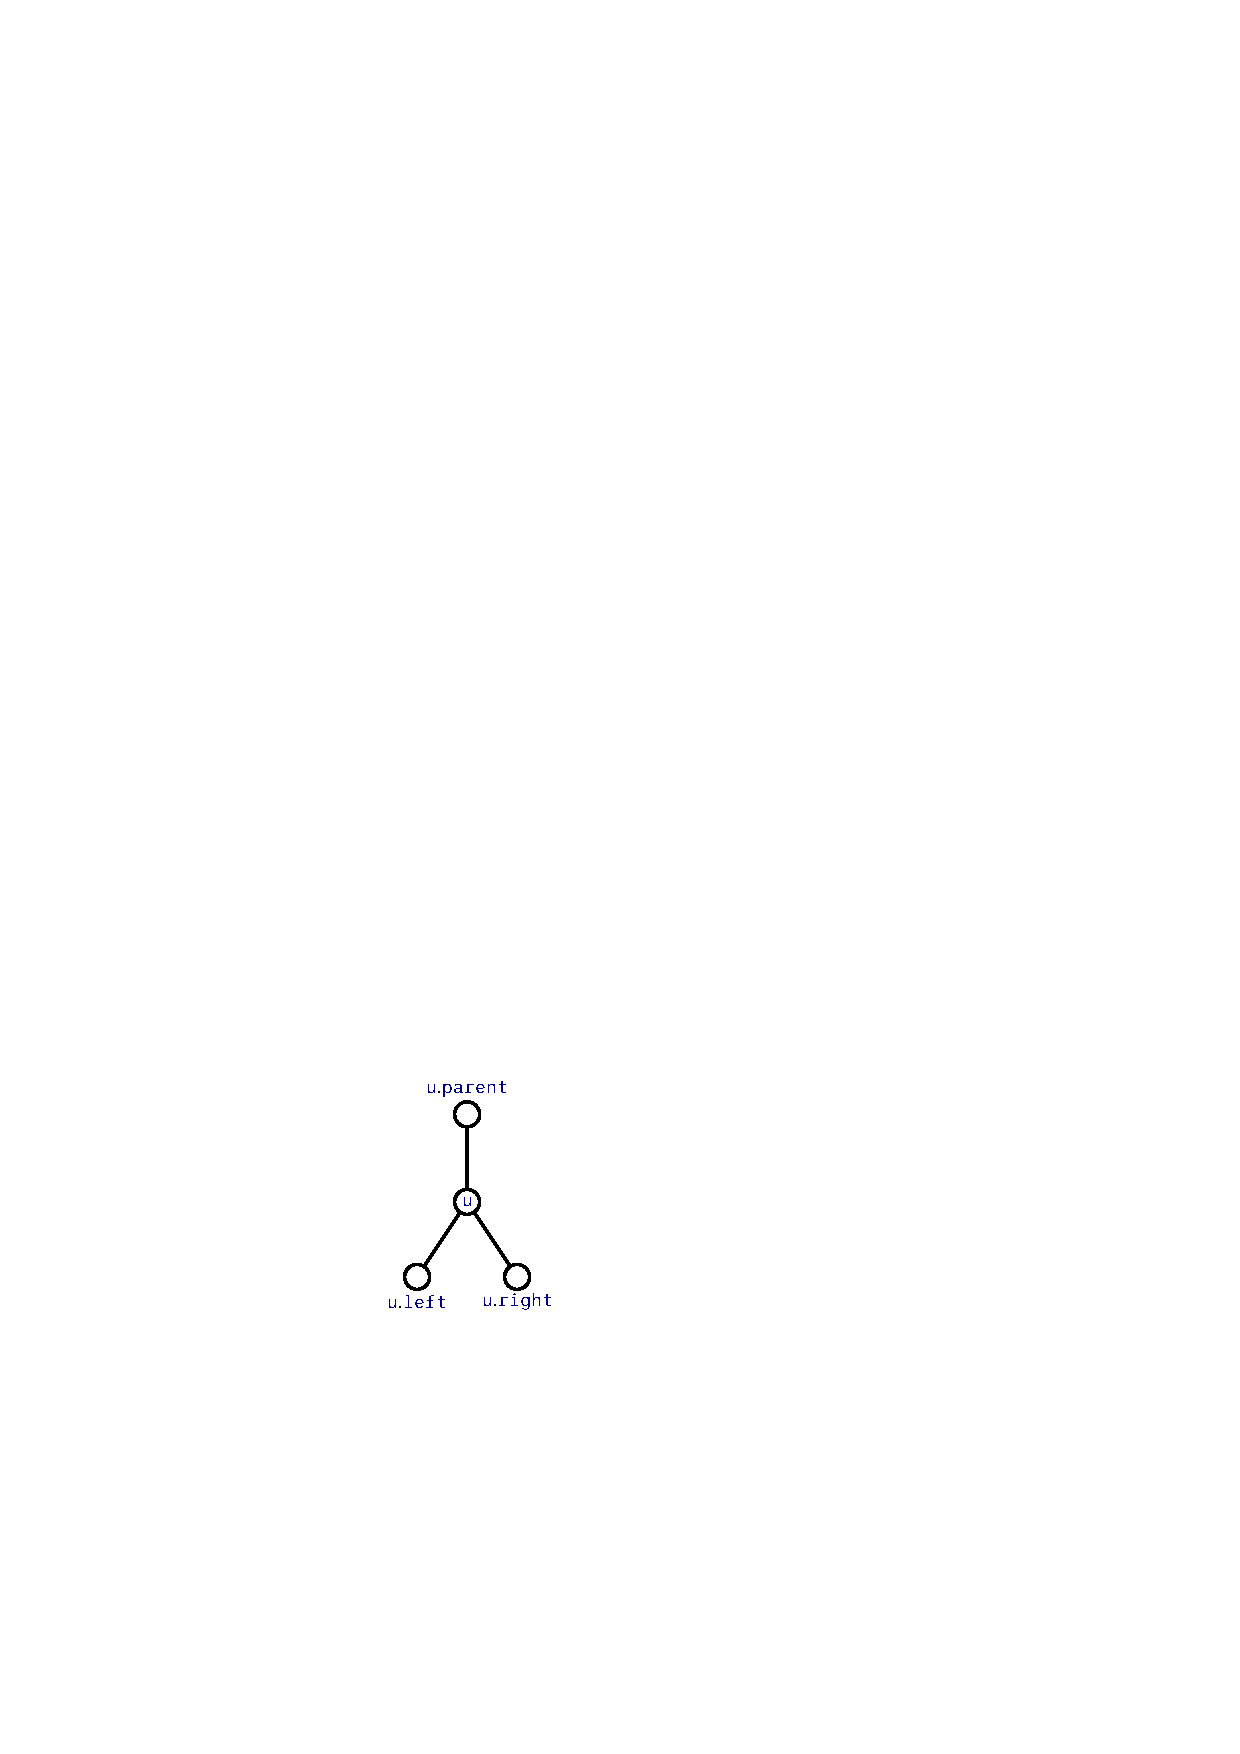
\includegraphics[scale=0.90909]{figs/bintree-traverse-1} 
  \end{center}
  \caption[Pai e filhos esquerdo e direito]{O pai, o filho esquerdo e o filho direito do nó  #u#
    em uma #ArvoreBinaria#.}
  \figlabel{bintree-orientation}
\end{figure}


\begin{figure}
  \begin{center}
    \begin{tabular}{cc}
      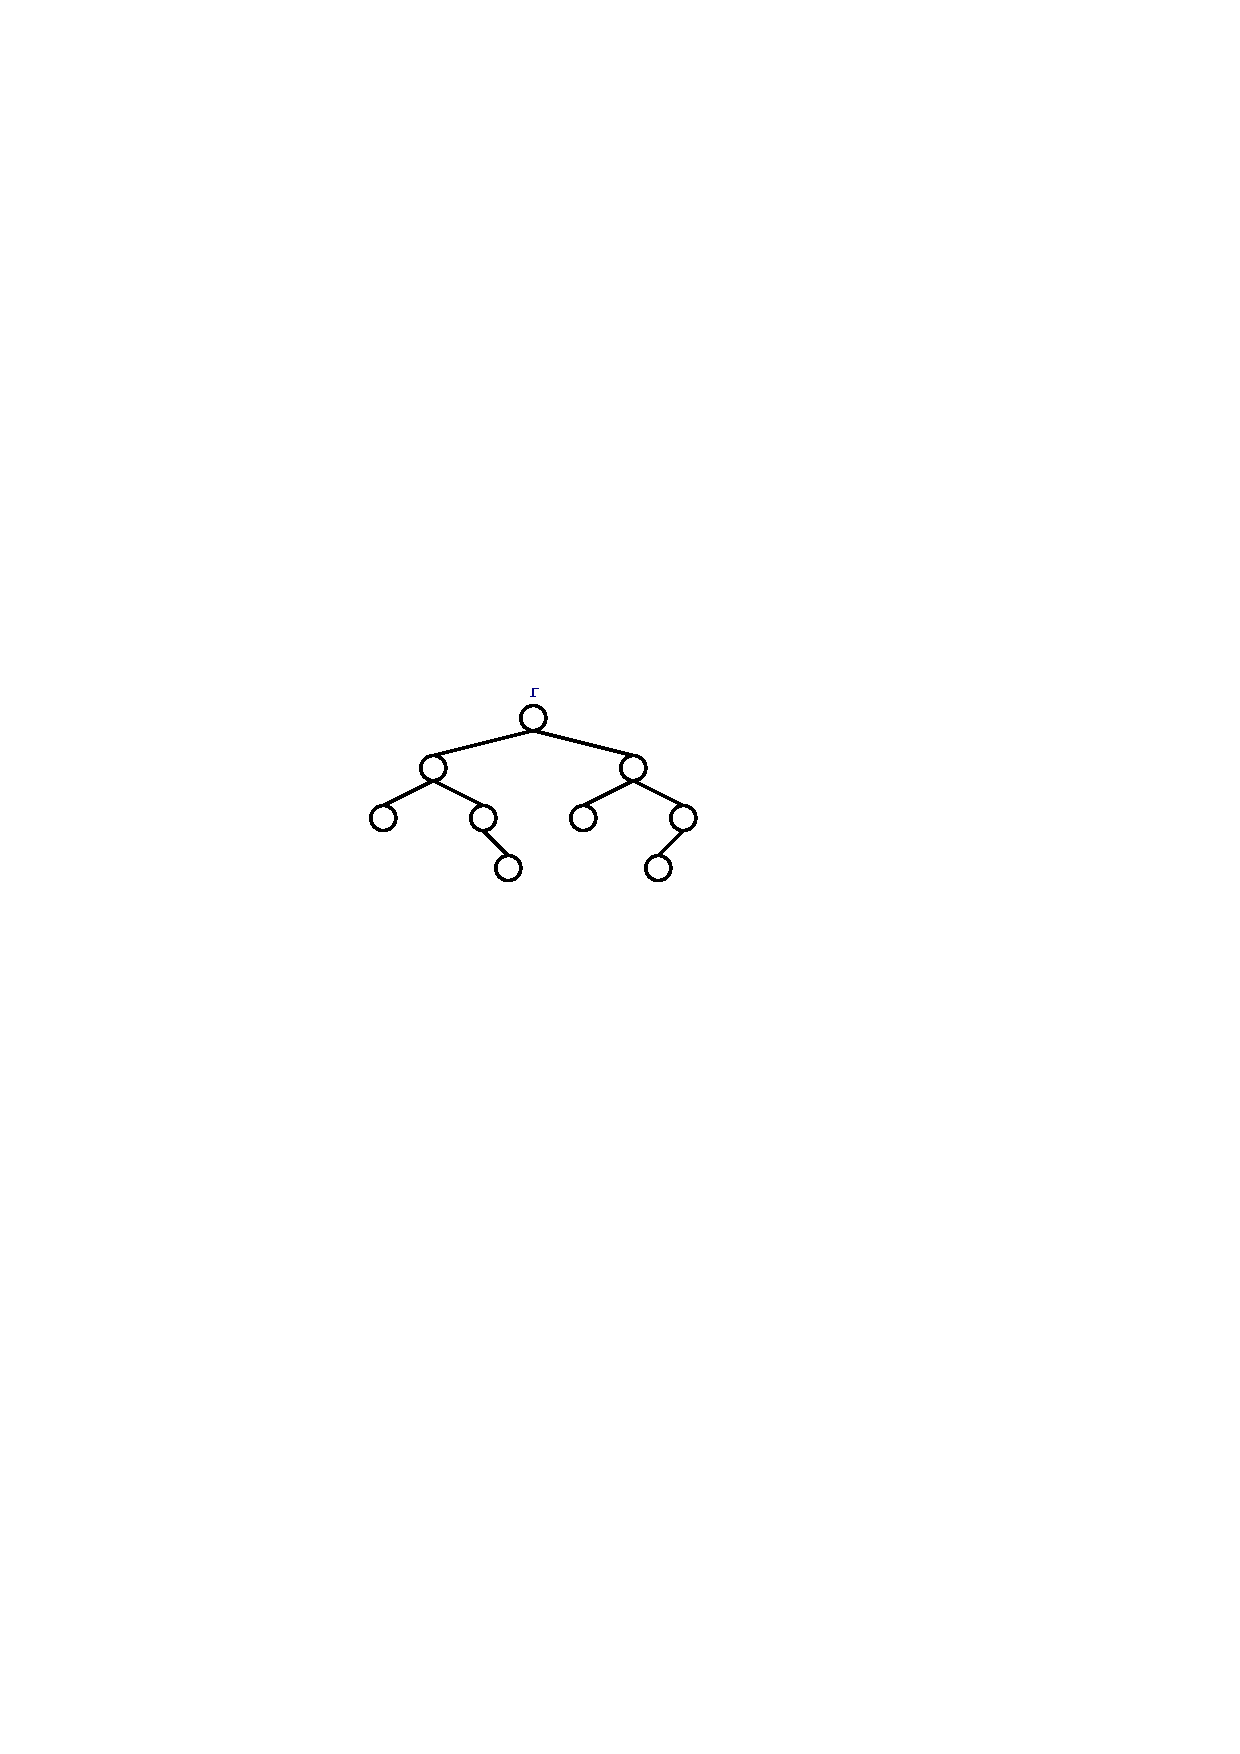
\includegraphics[width=\HalfScaleIfNeeded]{figs/bintree-1} &
      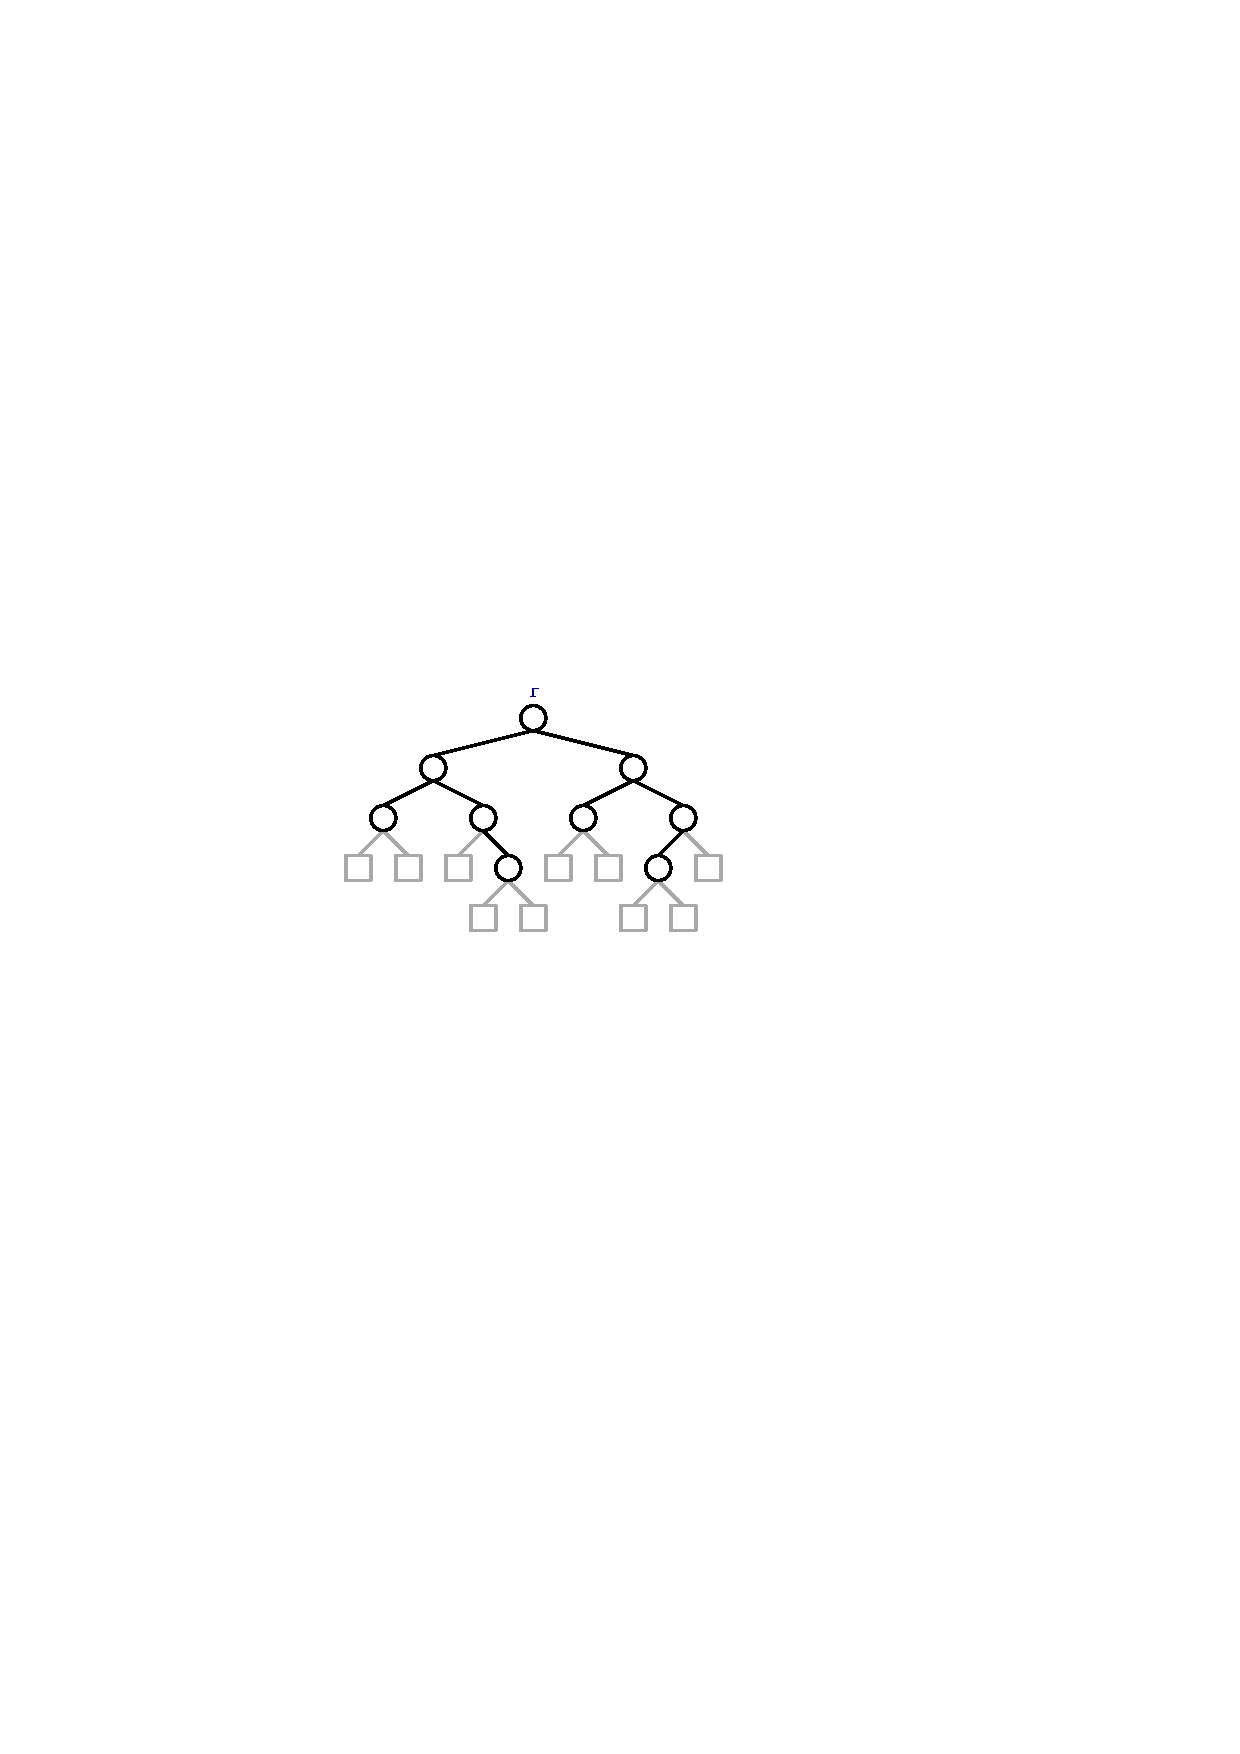
\includegraphics[width=\HalfScaleIfNeeded]{figs/bintree-2} \\
      (a) & (b)
    \end{tabular}
  \end{center}
  \caption{Uma árvore binária com (a)~nove nós reais e (b)~dez nós externos.}
  \figlabel{binary-tree}
\end{figure}

As árvores binárias são tão importantes que foi criada uma terminologia para elas: 
a \emph{profundidade}
\index{profundidade}%
de um nó, #u#, em uma árvore binária é o comprimento do caminho de #u# até a raiz da árvore.   Se um nó, #w#,
está no caminho de #u# até #r#, então #w# é chamado de \emph{ancestral}
\index{ancestral}%
de #u# e #u# um \emph{descendente}
\index{descendente}%
de #w#.  A \emph{subárvore} de um
nó, #u#, é uma árvore binária com raiz em #u# e contém todos
os descendentes de #u#.  A \emph{altura}
\index{altura!em uma árvore} de um nó, #u#, é o comprimento
do percurso mais longo entre #u# e um dos seus descendentes.  A \emph{altura} de
\index{altura!de uma árvore}%
uma árvore é a altura de sua raiz.
Um nó, #u#, é uma \emph{folha}
\index{folha}%
se ele não possui filhos.

Algumas vezes pensamos a árvore como se ela fosse expandida com \emph{nós externos}. Qualquer nó que não possua um filho esquerdo possui um nó externo
como seu filho esquerdo e, da mesma maneira, qualquer nó que não tenha um filho direito possui um nó externo como seu filho direito (veja 
\figref{binary-tree}.b). É fácil verificar, por indução, que uma
árvore binária com $#n#\ge 1$ nós reais possui $#n#+1$ nós externos.


\section{#ArvoreBinaria#: Uma Árvore Binária Básica}

\index{ArvoreBinaria@#ArvoreBinaria#}%
Um modo simples de representar um nó, #u#, em uma árvore binária é armazenar explicitamente, e no máximo, três vizinhos de #u#\notpcode{:}\pcodeonly{.}
\javaimport{ods/BinaryTree.BTNode<Node}
\cppimport{ods/BinaryTree.BTNode}
Quando um dos três vizinhos não está presente, atribuímos a ele o valor #nil#.
Deste modo, ambos os nós externos da árvore e o pai da raiz correspondem ao valor #nil#.

A própria árvore binária pode ser representada por uma
\javaonly{referência}\cpponly{ponteiro}\pcodeonly{referência} ao seu nó raiz, #r#:
\codeimport{ods/BinaryTree.r}

Podemos calcular a profundidade de um nó, #u#, em uma árvore binária contando
o número de passos no caminho de #u# até a raiz:
\codeimport{ods/BinaryTree.depth(u)}


\subsection{Algoritmos Recursivos}

\index{algoritmo recursivo}%
Usar algoritmos recursivos torna muito fácil o cálculo envolvendo árvores binárias. Por exemplo, para calcular o tamanho (número de nós) de uma
árvore binária com raízes no nó #u#, recursivamente calculamos o tamanho
das duas subárvores com raiz nos filhos de #u#, somamos os tamanhos e adicionamos um:

\codeimport{ods/BinaryTree.size(u)}

Para calcular a altura de um nó #u#, podemos calcular a altura das duas subárvores de #u#, pegar o valor máximo e adicionar 1:

\codeimport{ods/BinaryTree.height(u)}

\subsection{Percurso em Árvores Binárias}
\seclabel{bintree:traversal}

\index{percurso!de uma árvore binária}%
\index{percurso em árvore}%
\index{percurso em árvore-binária}%
Ambos os algoritmos da seção anterior usam a recursão para visitar
todos os nós de uma árvore binária.  Cada um deles visita os nós da
árvore binária na mesma ordem que o seguinte código:
\codeimport{ods/BinaryTree.traverse(u)}

O uso da recursão neste caso produz um código bem sucinto e simples, porém ele pode ser
também problemático.  A profundidade máxima da recursão é dada pela
profundidade máxima do nó na árvore binária, i.e., a altura da árvore.
Se a altura da árvore é muito grande, então essa recursão pode muito bem utilizar mais espaço da pilha do que esteja disponível, causando um fechamento do programa.

Para percorrer uma árvore binária sem utilizar a recursão, você pode usar um algoritmo que
se baseie de onde ele vem para saber para onde vai.  Veja a
\figref{bintree-traverse}.  Se chegamos ao nó #u# a partir de #u.pai#,
então a próxima coisa a ser feita é visitar #u.esquerdo#.  Se chegamos a #u#
por #u.esquerdo#, então a próxima coisa a ser feita é visitar #u.direito#.  Se chegamos 
em #u# por #u.direito#, então terminamos de visitar a subárvore de #u#,
e retornamos para #u.pai#.  O código seguinte implementa esta ideia, com o código incluído para lidar com os casos em que qualquer um de #u.esquerdo#,
#u.direito#, ou #u.pai# seja #nil#:
\codeimport{ods/BinaryTree.traverse2()}

\begin{figure}
  \begin{center}
    \begin{tabular}{cc}
      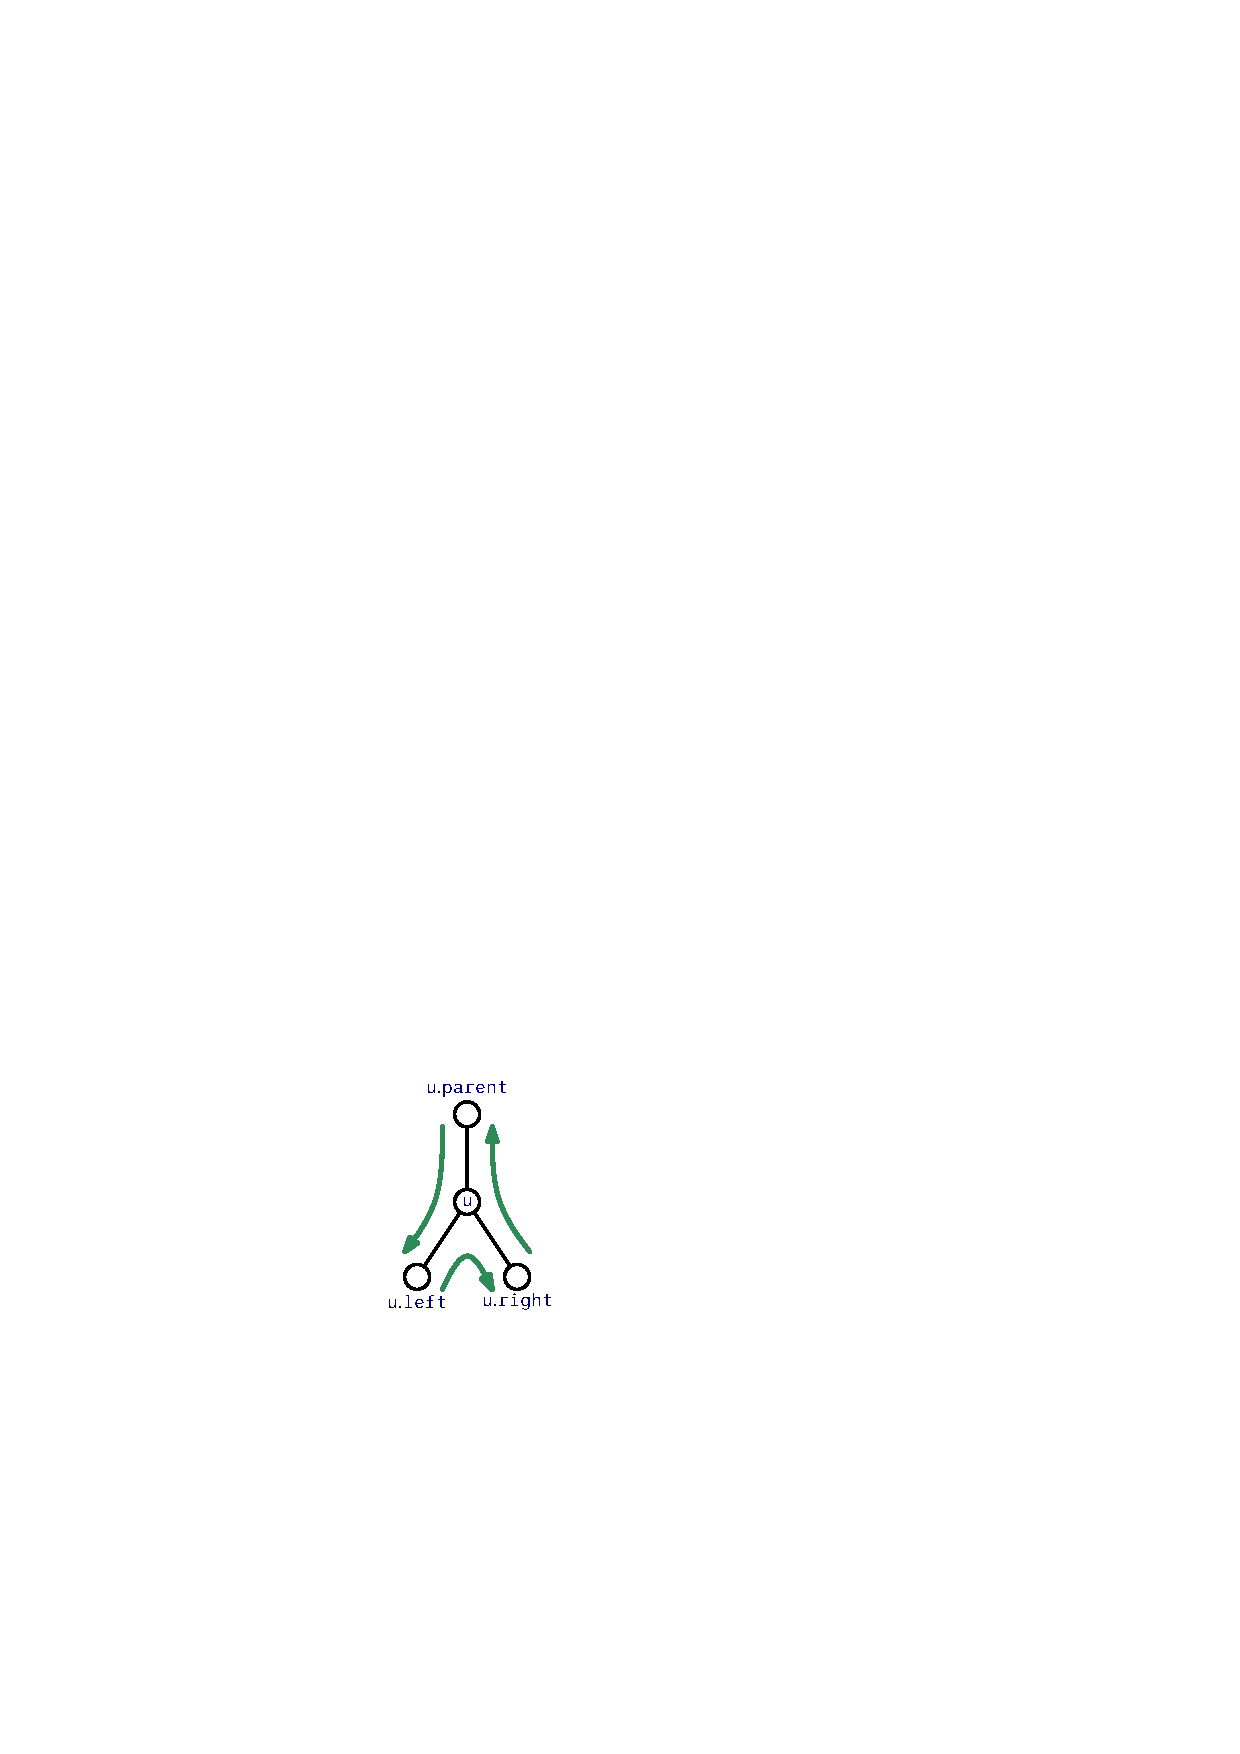
\includegraphics[scale=0.90909]{figs/bintree-traverse-2}
      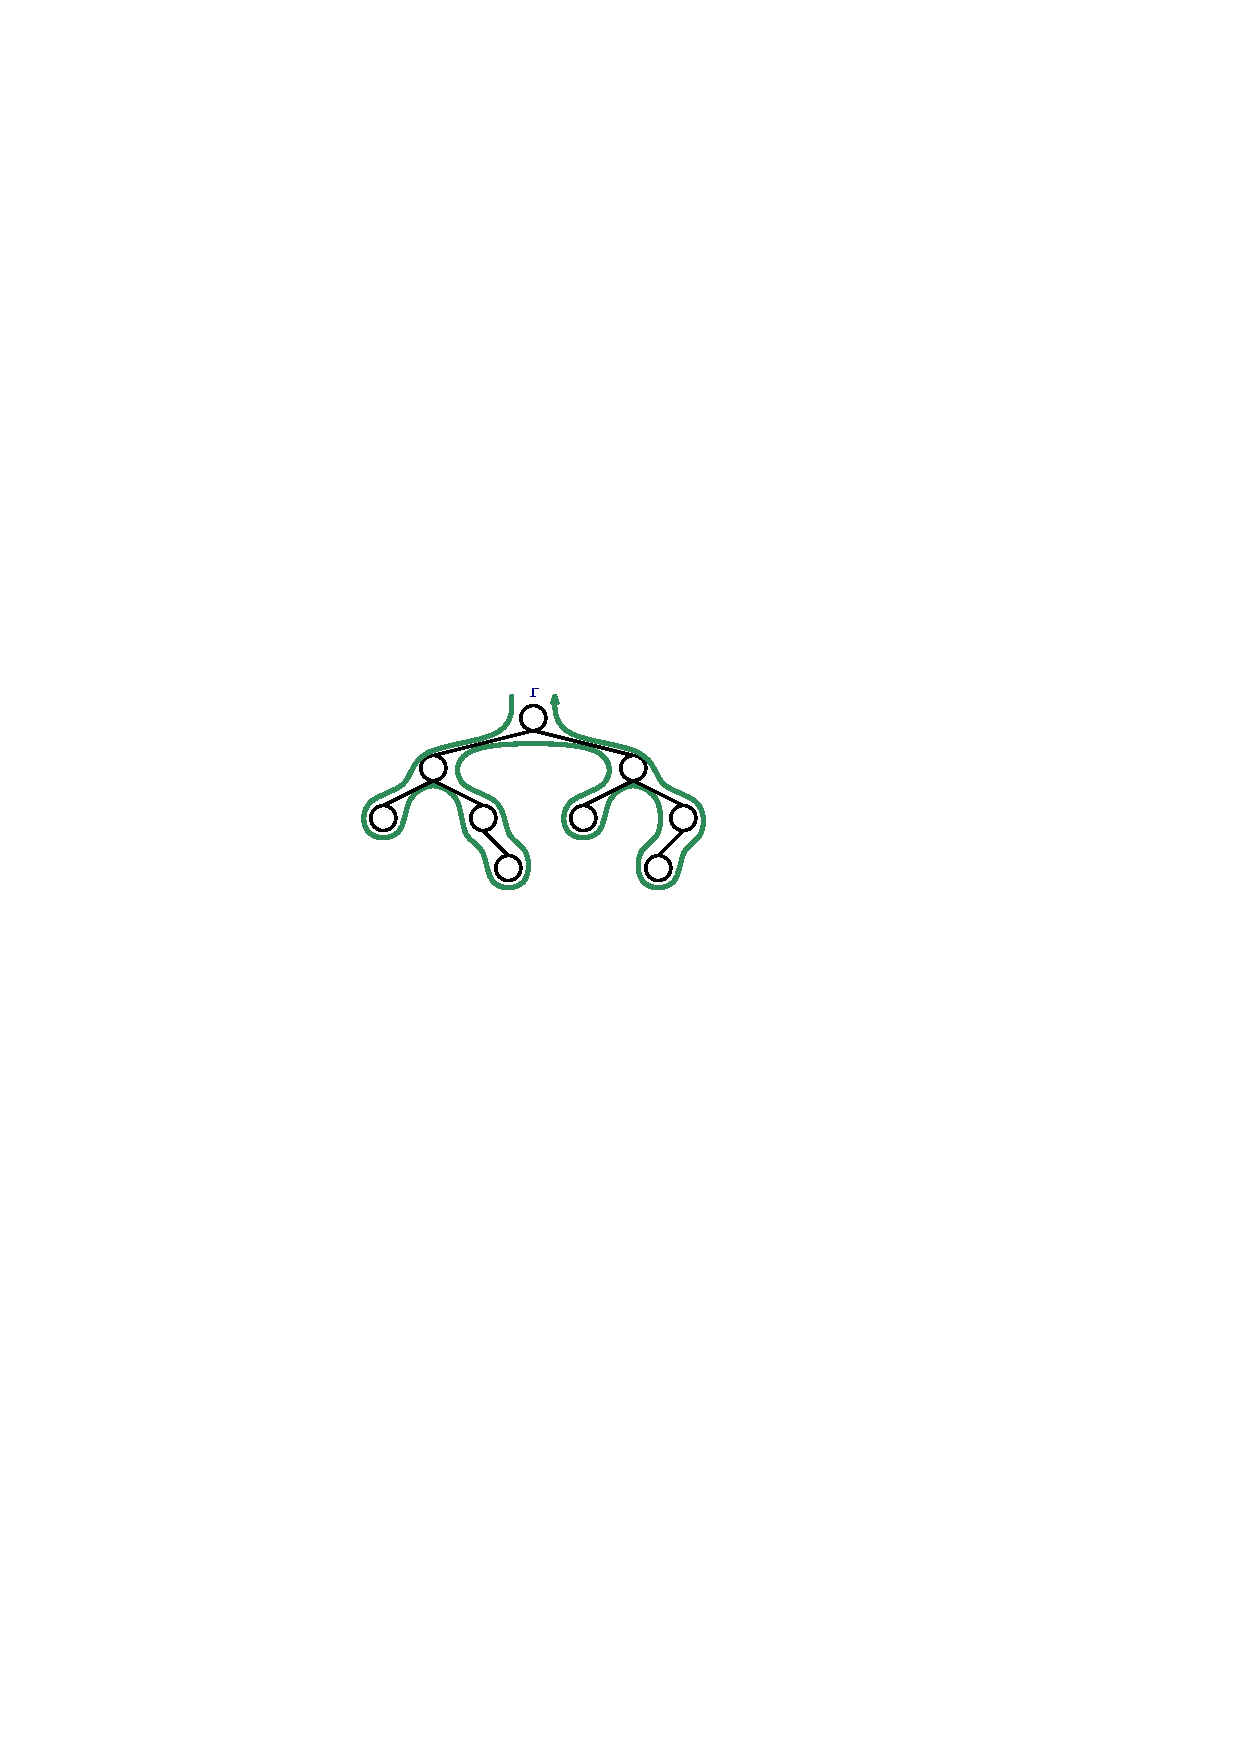
\includegraphics[scale=0.90909]{figs/bintree-3}
    \end{tabular}
  \end{center}
  \caption[Percorrendo uma ArvoreBinaria]{Os três casos que ocorrem no nó
    #u# quando percorremos uma árvore binária não recursivamente, e o resultado da travessia pela árvore.}
  \figlabel{bintree-traverse}
\end{figure}

Os mesmos resultados que podem ser obtidos usando a recursão também podem ser obtidos desta maneira, sem recursão. Por exemplo, para calcular o tamanho 
da árvore mantemos um contador, #n#, e incrementamos #n# sempre que visitamos um nó pela primeira vez:
\codeimport{ods/BinaryTree.size2()}

Em algumas implementações de árvore binárias, o campo #pai# não é usado.
Quando é este o caso, um implementação não recursiva ainda é possível,
porém a implementação deve usar uma #Lista# (ou #Pilha#) para acompanhar
o caminho do nó atual até a raiz.

Um tipo especial de percurso que não cabe no padrão das funções acima é o \emph{percurso em profundidade}.
\index{percurso em profundidade}%
\index{percurso!profundidade}%
Em um percurso em profundidade, os nós são visitados nível por nível, começando pela raiz e indo para baixo, visitando os nós de cada nível, da esquerda para a direita
(veja
\figref{bintree-bfs}). Isto é similar ao modo pelo qual lemos um texto em português.   O percurso em profundidade é implementado usando uma fila, #q#, que inicialmente contém apenas a raiz, #r#.  Em cada passo,
extraímos o próximo nó, #u#, de #q#, processamos #u# e adicionamos #u.esquerdo#
e #u.direito# (se eles não são #nil#) a #q#:
\codeimport{ods/BinaryTree.bfTraverse()}

\begin{figure}
  \begin{center}
    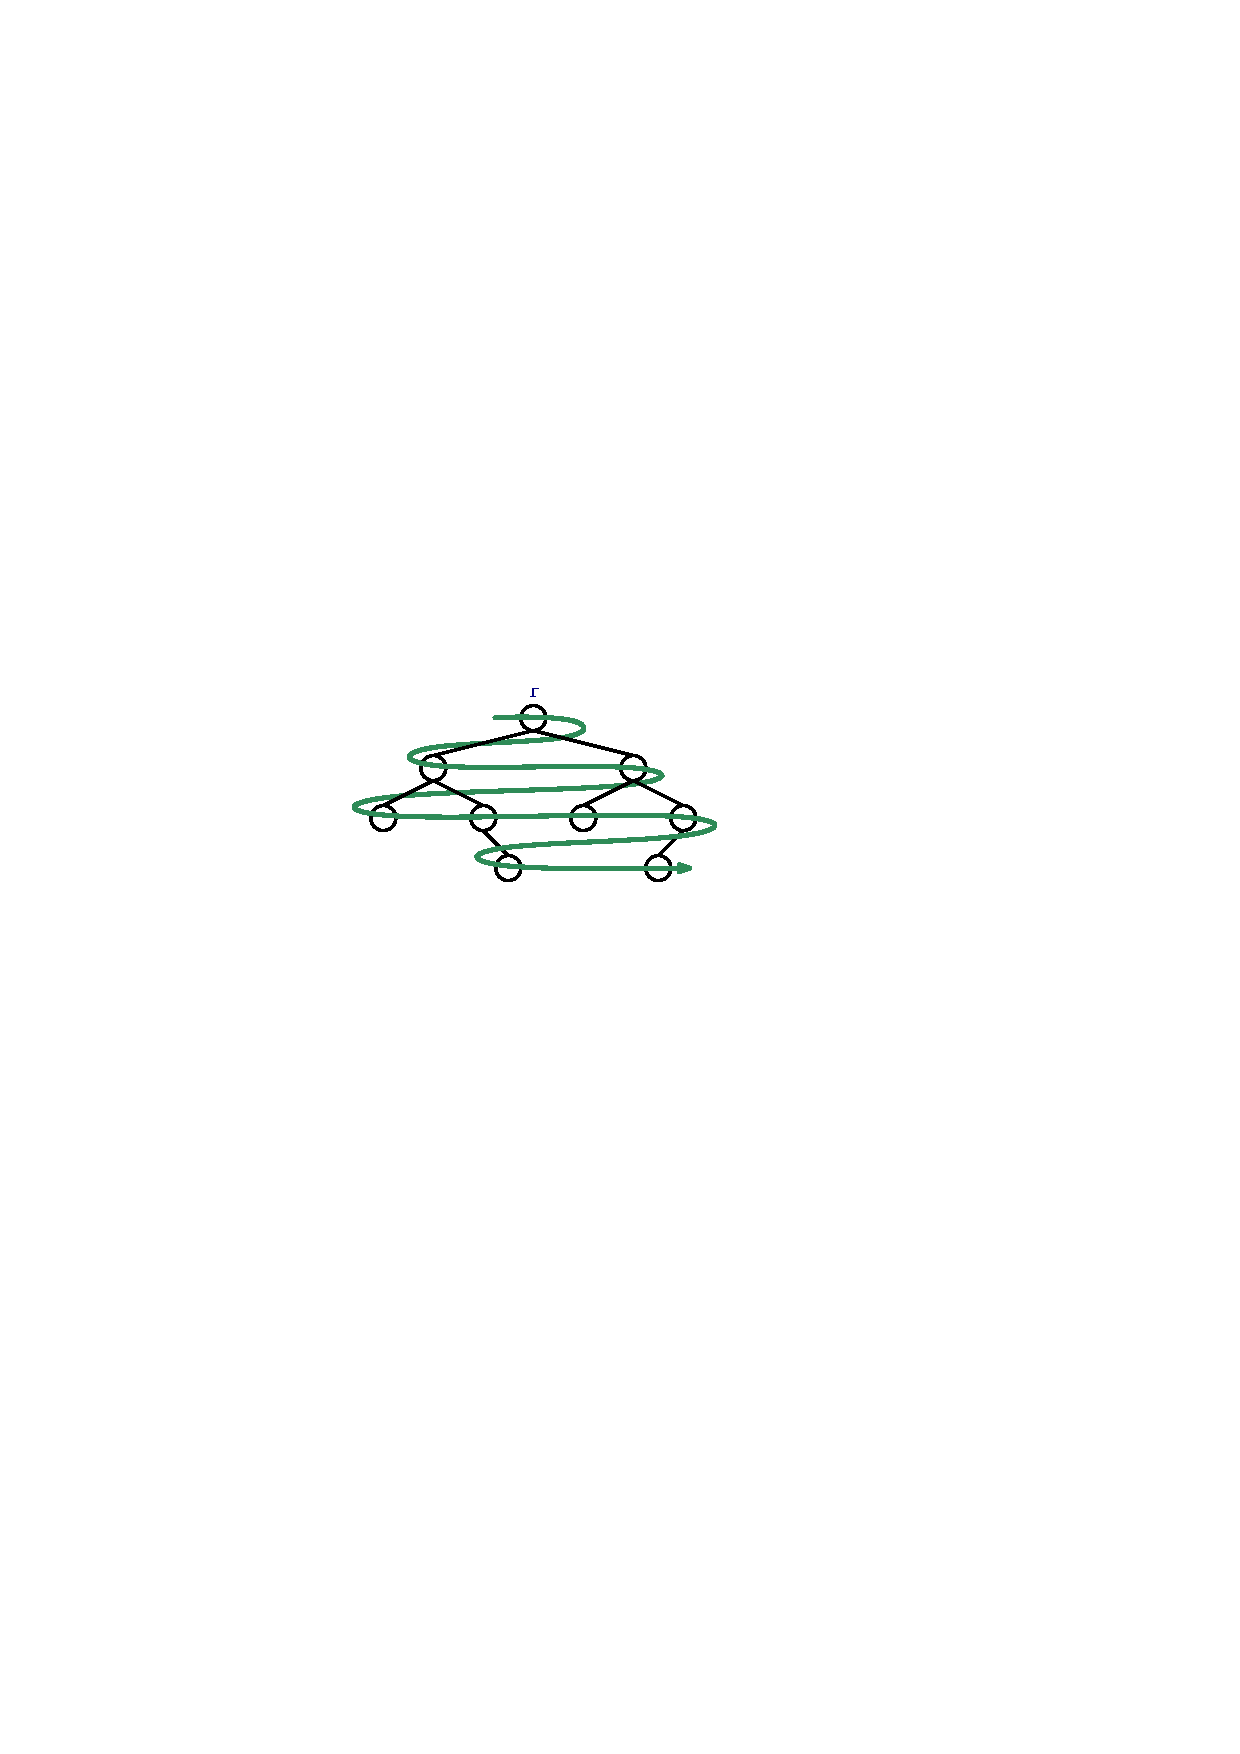
\includegraphics[scale=0.90909]{figs/bintree-4}
  \end{center}
  \caption{Durante um percurso em profundidade, os nós de uma árvore binária são visitados nível por nível e da esquerda para a direita dentro de cada nível.}
  \figlabel{bintree-bfs}
\end{figure}





\section{#ArvoreBinariaDeBusca#: Uma Árvore Binária de Busca não Balanceada}
\seclabel{binarysearchtree}

\index{ArvoreBinariaDeBusca@#ArvoreBinariadeBusca#}%
\index{árvore binária de busca}%
\index{árvore binária!busca}%
Uma #ArvoreBinariaDeBusca# é um tipo especial de árvore binária na qual cada nó, #u#,
também armazena um valor, #u.x#, de uma ordem total.  Os valores em uma árvore binária de busca obedece à \emph{propriedade da árvore binária de busca}:
\index{árvore binária de busca}%
para um nó, #u#, cada valor armazenado na subárvore com raiz em #u.esquerdo# é menor que #u.x# e cada valor armazenado na subárvore com raiz em
#u.direito# é maior que #u.x#.  Um exemplo de uma #ArvoreBinariaDeBusca# é mostrado na \figref{bst}.

\begin{figure}
  \begin{center}
    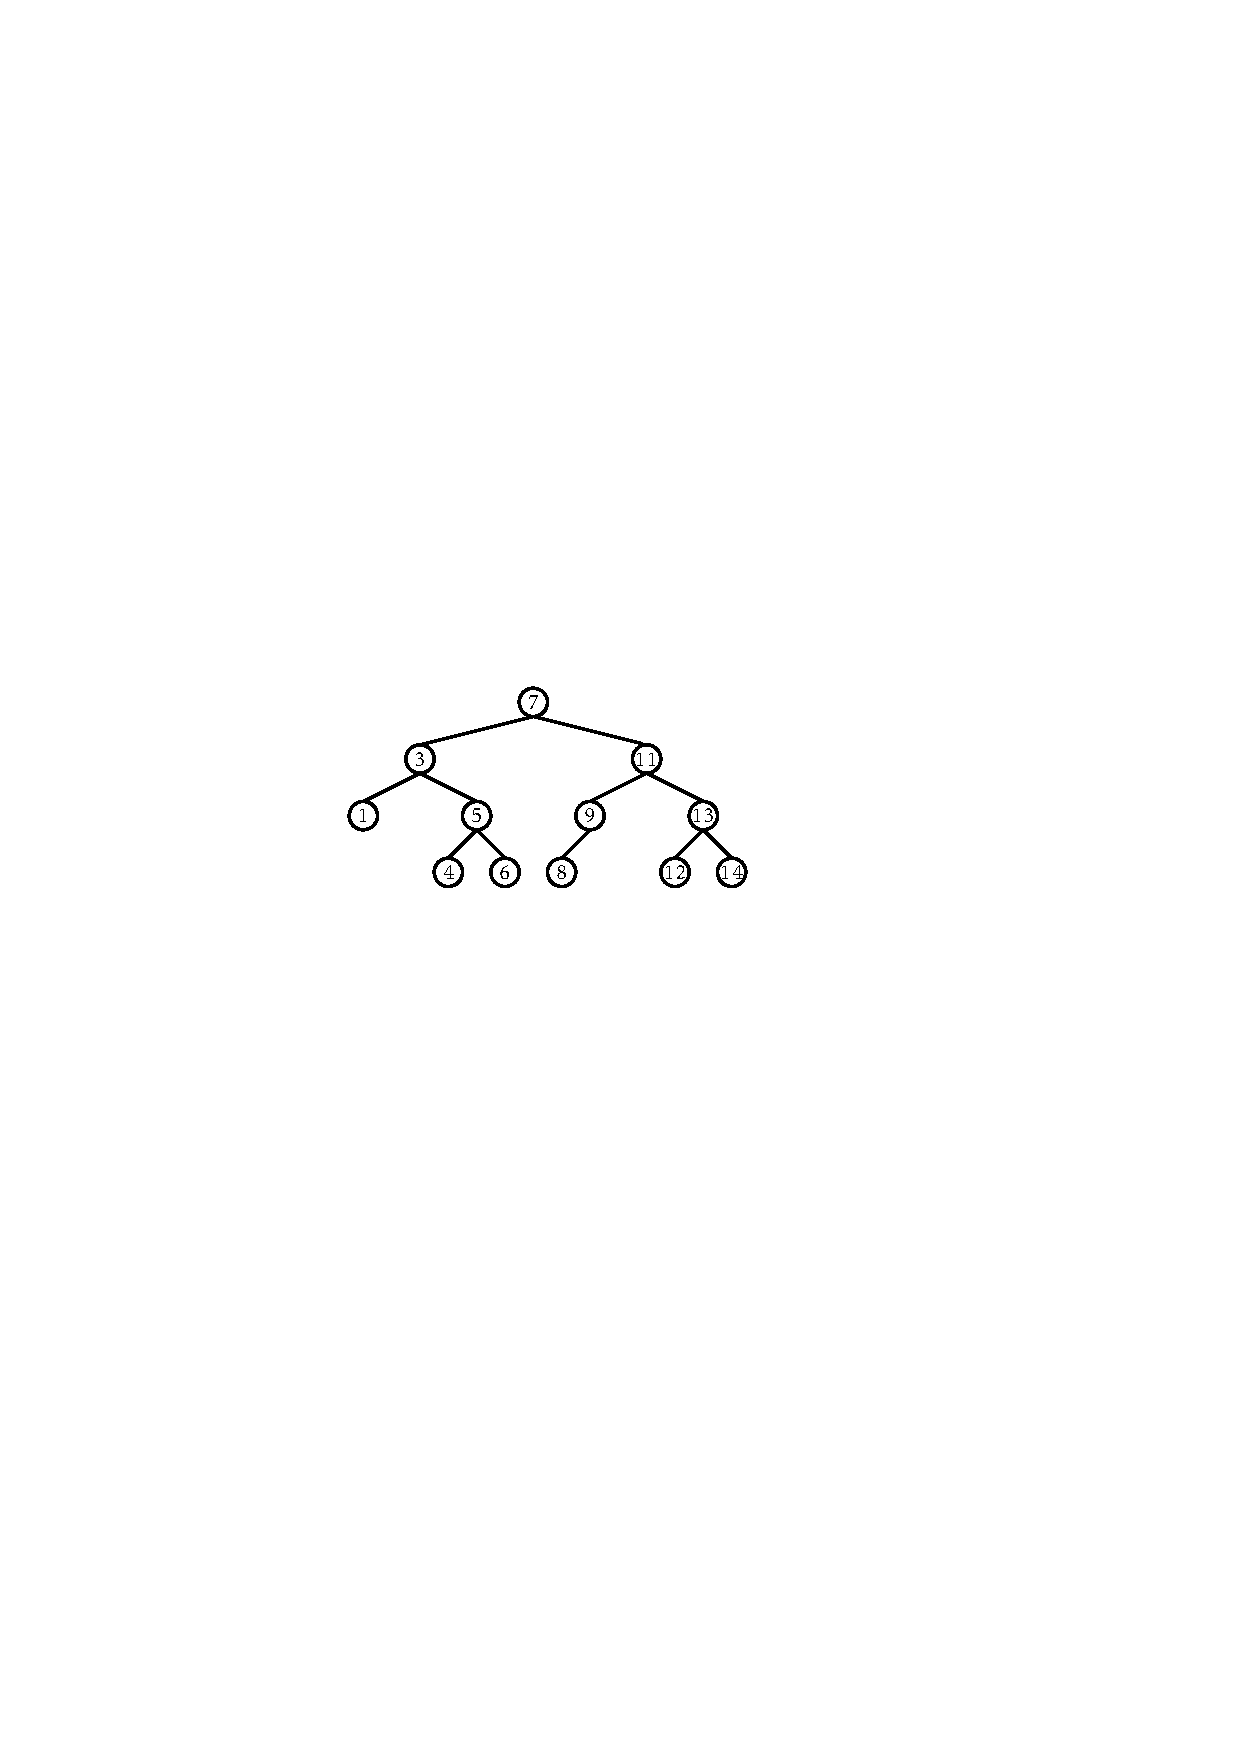
\includegraphics[scale=0.90909]{figs/bst-example}
    %\includegraphics[scale=0.90909]{figs/binary-tree-4}
  \end{center}
  \caption{Uma árvore binária de busca.}
  \figlabel{bst}
\end{figure}


\subsection{Busca}

\index{caminho de busca!em uma árvore binária de busca}%
A propriedade da árvore binária de busca é extremamente útil porque ela permite localizar rapidamente um valor, #x#, dentro da árvore binária de busca.  Para isto, começamos procurando por #x# na raiz, #r#. Quando examinamos um nó, #u#, podem ocorrer três casos:
\begin{enumerate}
\item Se $#x#< #u.x#$, então a procura continua em #u.esquerdo#;
\item Se $#x#> #u.x#$, então a procura continua em #u.direito#;
\item Se $#x#= #u.x#$, então encontramos o nó #u# que contém #x#.
\end{enumerate}
A busca termina quando o Caso~3 ocorre ou quando #u=nil#.  No primeiro caso, encontramos #x#.  No último caso, concluímos que #x#
não está na árvore binária de busca.
\codeimport{ods/BinarySearchTree.findEQ(x)}

Dois exemplos de busca em uma árvore binária de busca são mostrados na 
\figref{bst-search}.  Como é mostrado no segundo exemplo, mesmo se não encontramos #x# na árvore, ainda obtemos alguma informação valiosa.  Se olhamos para o último nó, #u#, no qual o Caso~1 ocorre, percebemos que #u.x# é o menor valor na árvore que é maior que #x#.  De modo análogo,
o último nó no qual o Caso~2 ocorre contém o maior valor na árvore que é menor #x#.  Deste modo, guardando a informação do último nó, #z#, no qual o Caso~1 ocorre, uma #ArvoreBinariaDeBusca# pode implementar a operação #encontra(x)# que retorna o menor valor armazenado que é maior que ou igual a #x#:
\codeimport{ods/BinarySearchTree.find(x)}

\begin{figure}
  \begin{center}
    \begin{tabular}{cc}
    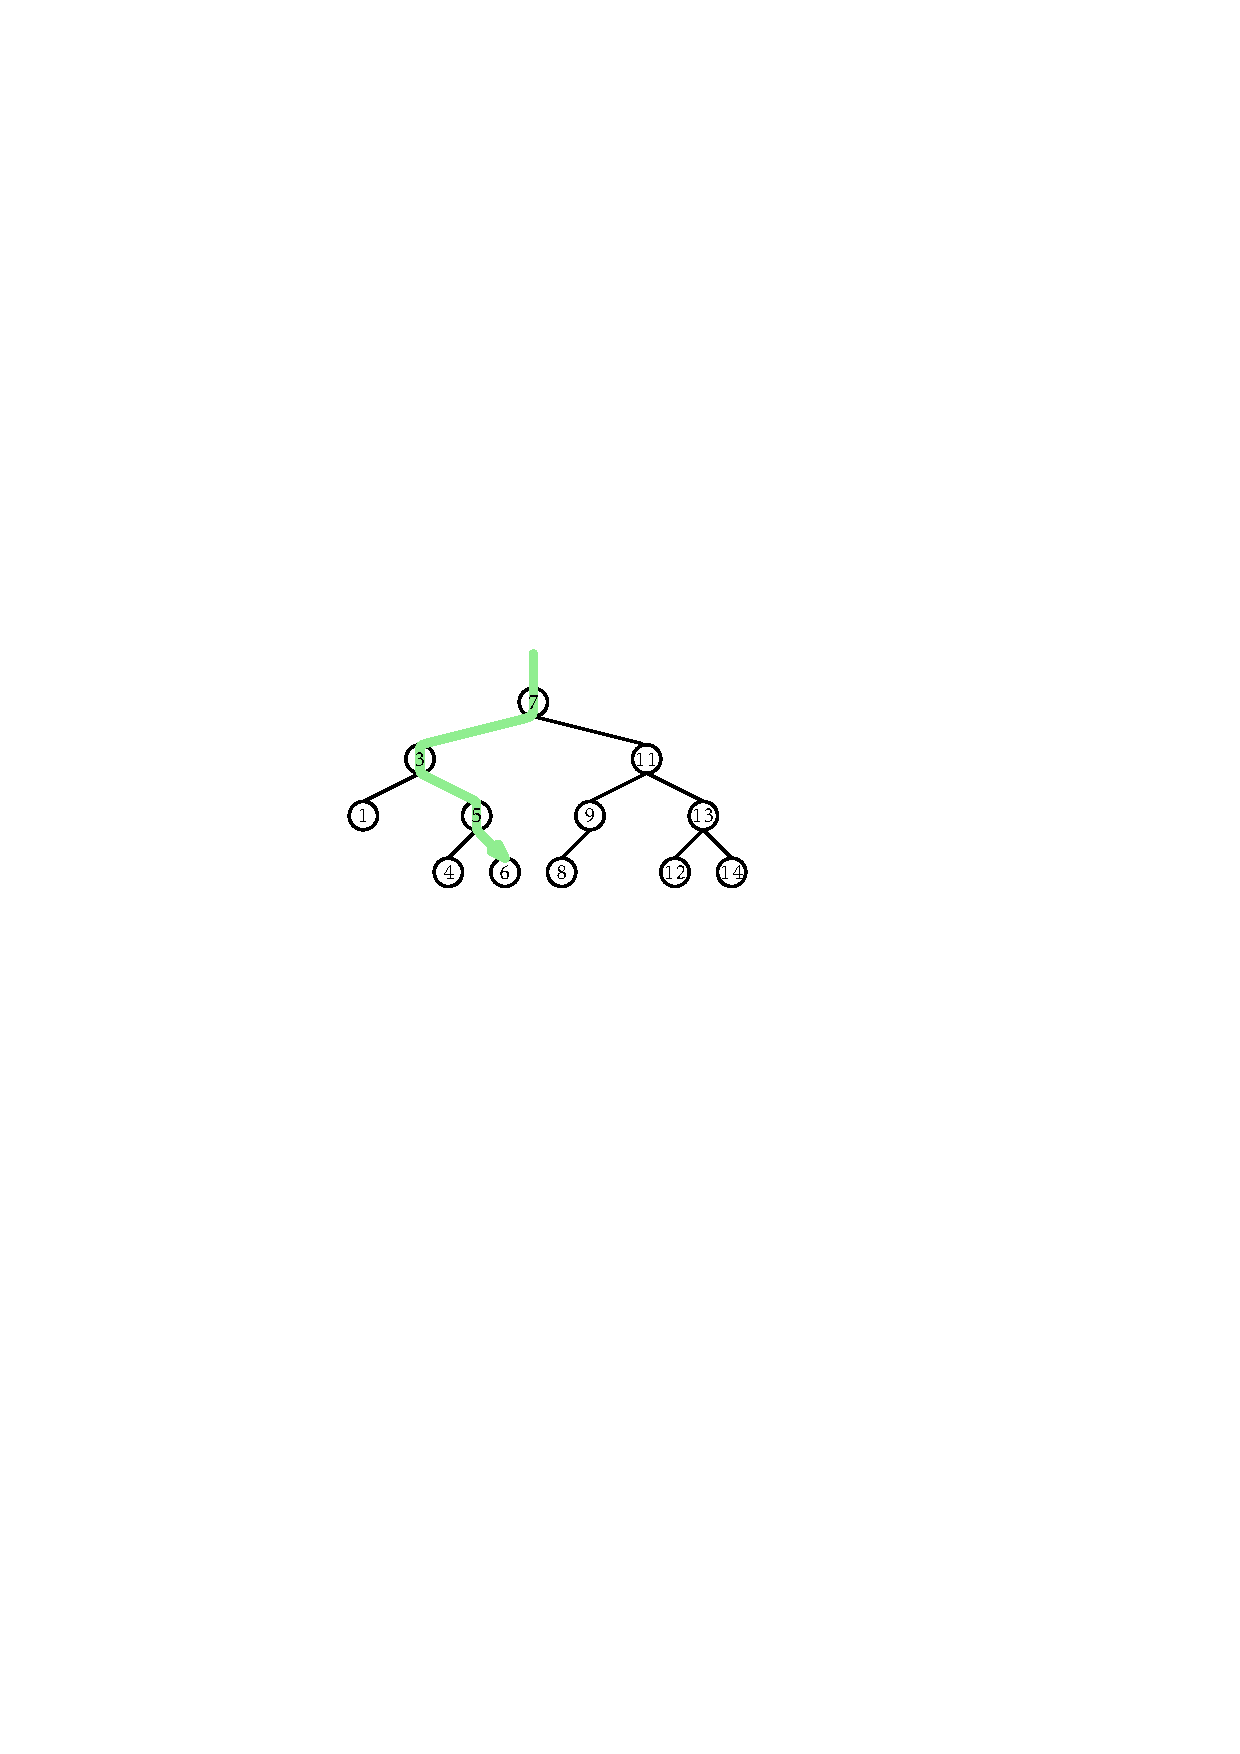
\includegraphics[width=\HalfScaleIfNeeded]{figs/bst-example-2} &
    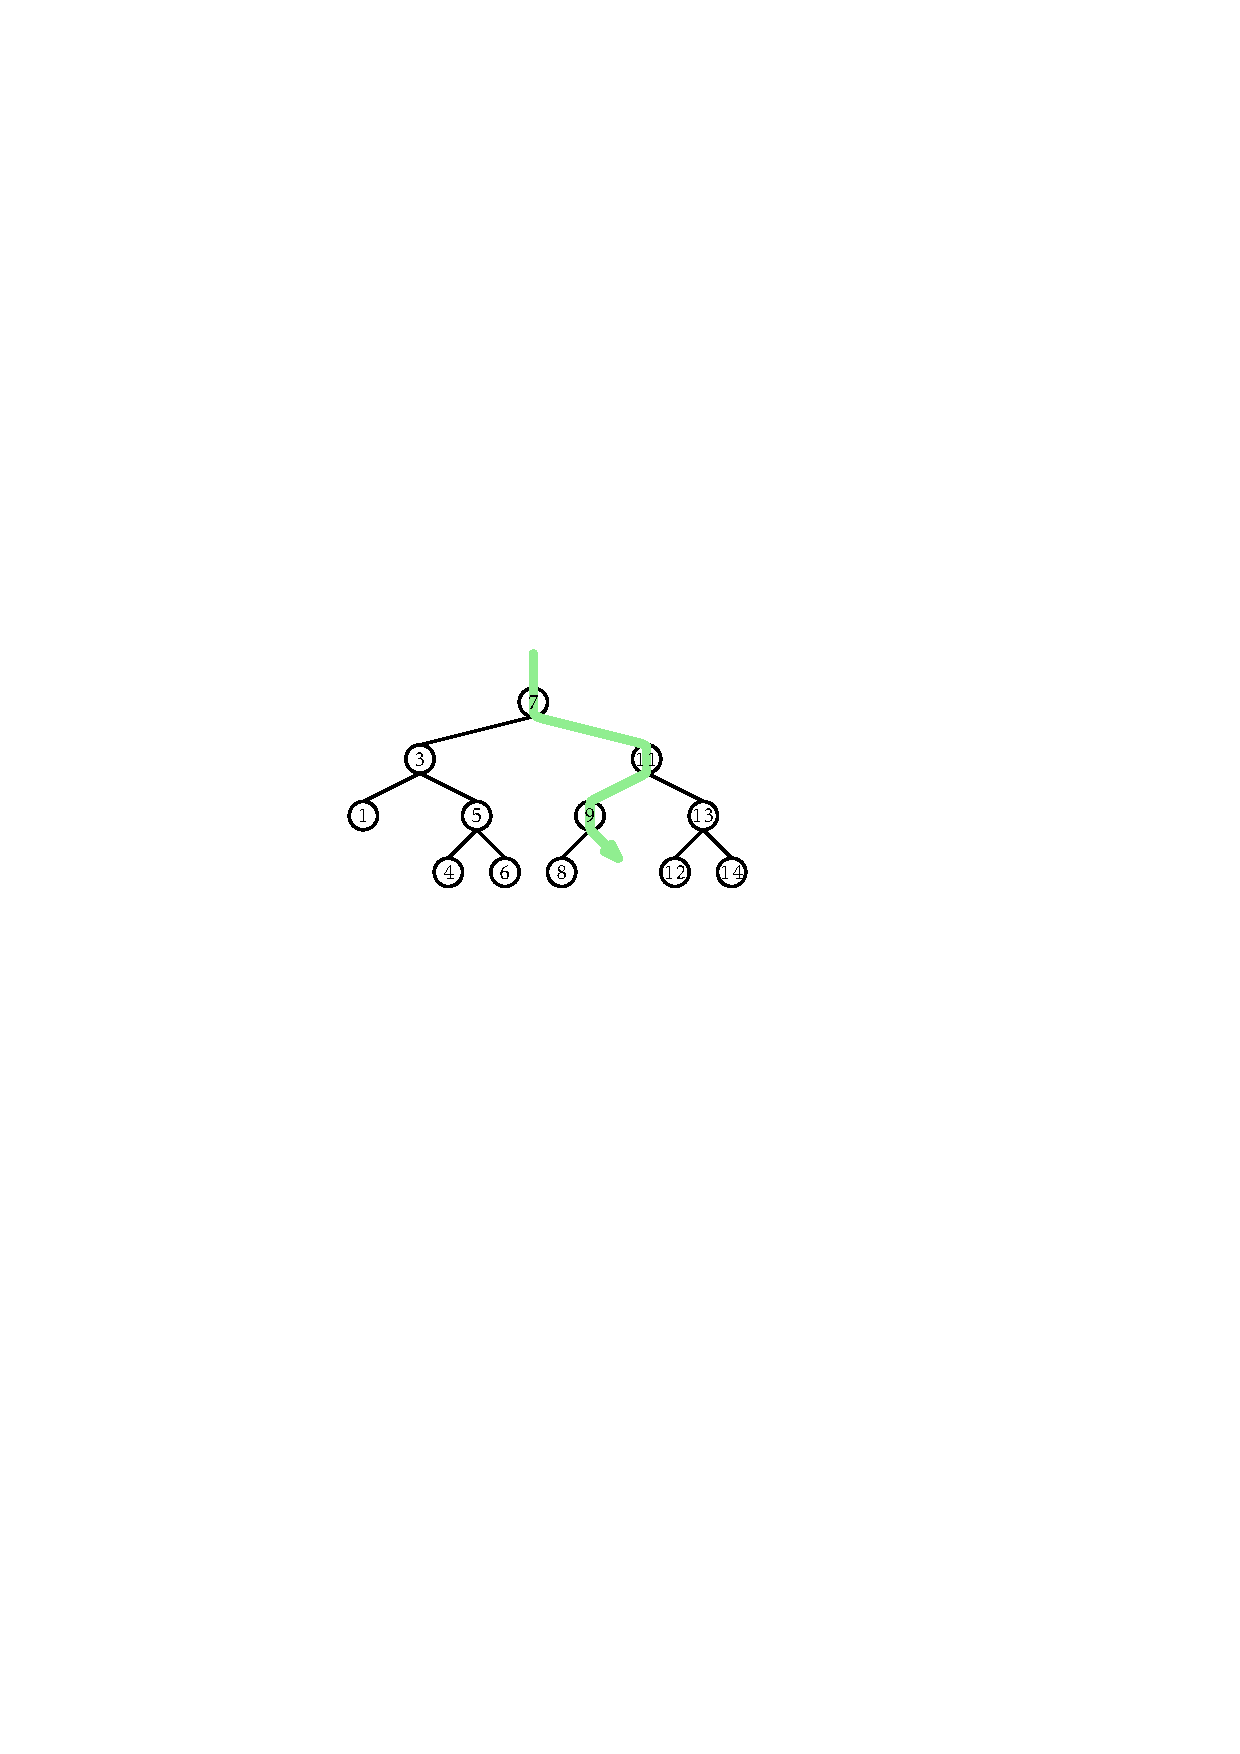
\includegraphics[width=\HalfScaleIfNeeded]{figs/bst-example-3} \\
    (a) & (b)
    \end{tabular}
  \end{center}
  \caption{Um exemplo de (a)~uma busca com sucesso (por $6$) e (b)~uma busca frustrada (por $10$) em uma árvore binária de busca.}
  \figlabel{bst-search}
\end{figure}


\subsection{Inserção}

Para inserir um novo valor, #x#, a uma #ArvoreBinariaDeBusca#, procuramos primeiro por #x#. Se o encontramos, então não precisamos inseri-lo.  Caso contrário, armazenamos #x# em um filho do último nó, #p#, encontrado durante a busca por #x#. Se o novo nó é o filho esquerdo ou direito de #p# depende do resultado da comparação de #x# e #p.x#.
\codeimport{ods/BinarySearchTree.add(x)}
\codeimport{ods/BinarySearchTree.findLast(x)}
\codeimport{ods/BinarySearchTree.addChild(p,u)}
Um exemplo é mostrado na \figref{bst-insert}. A parte que consome mais tempo neste processo é a busca inicial por #x#, que demanda um tempo proporcional à altura do nó recém adicionado #u#.
No pior caso, isto é igual à altura da #ArvoreBinariaDeBusca#.


\begin{figure}
  \begin{center}
    \begin{tabular}{cc}
    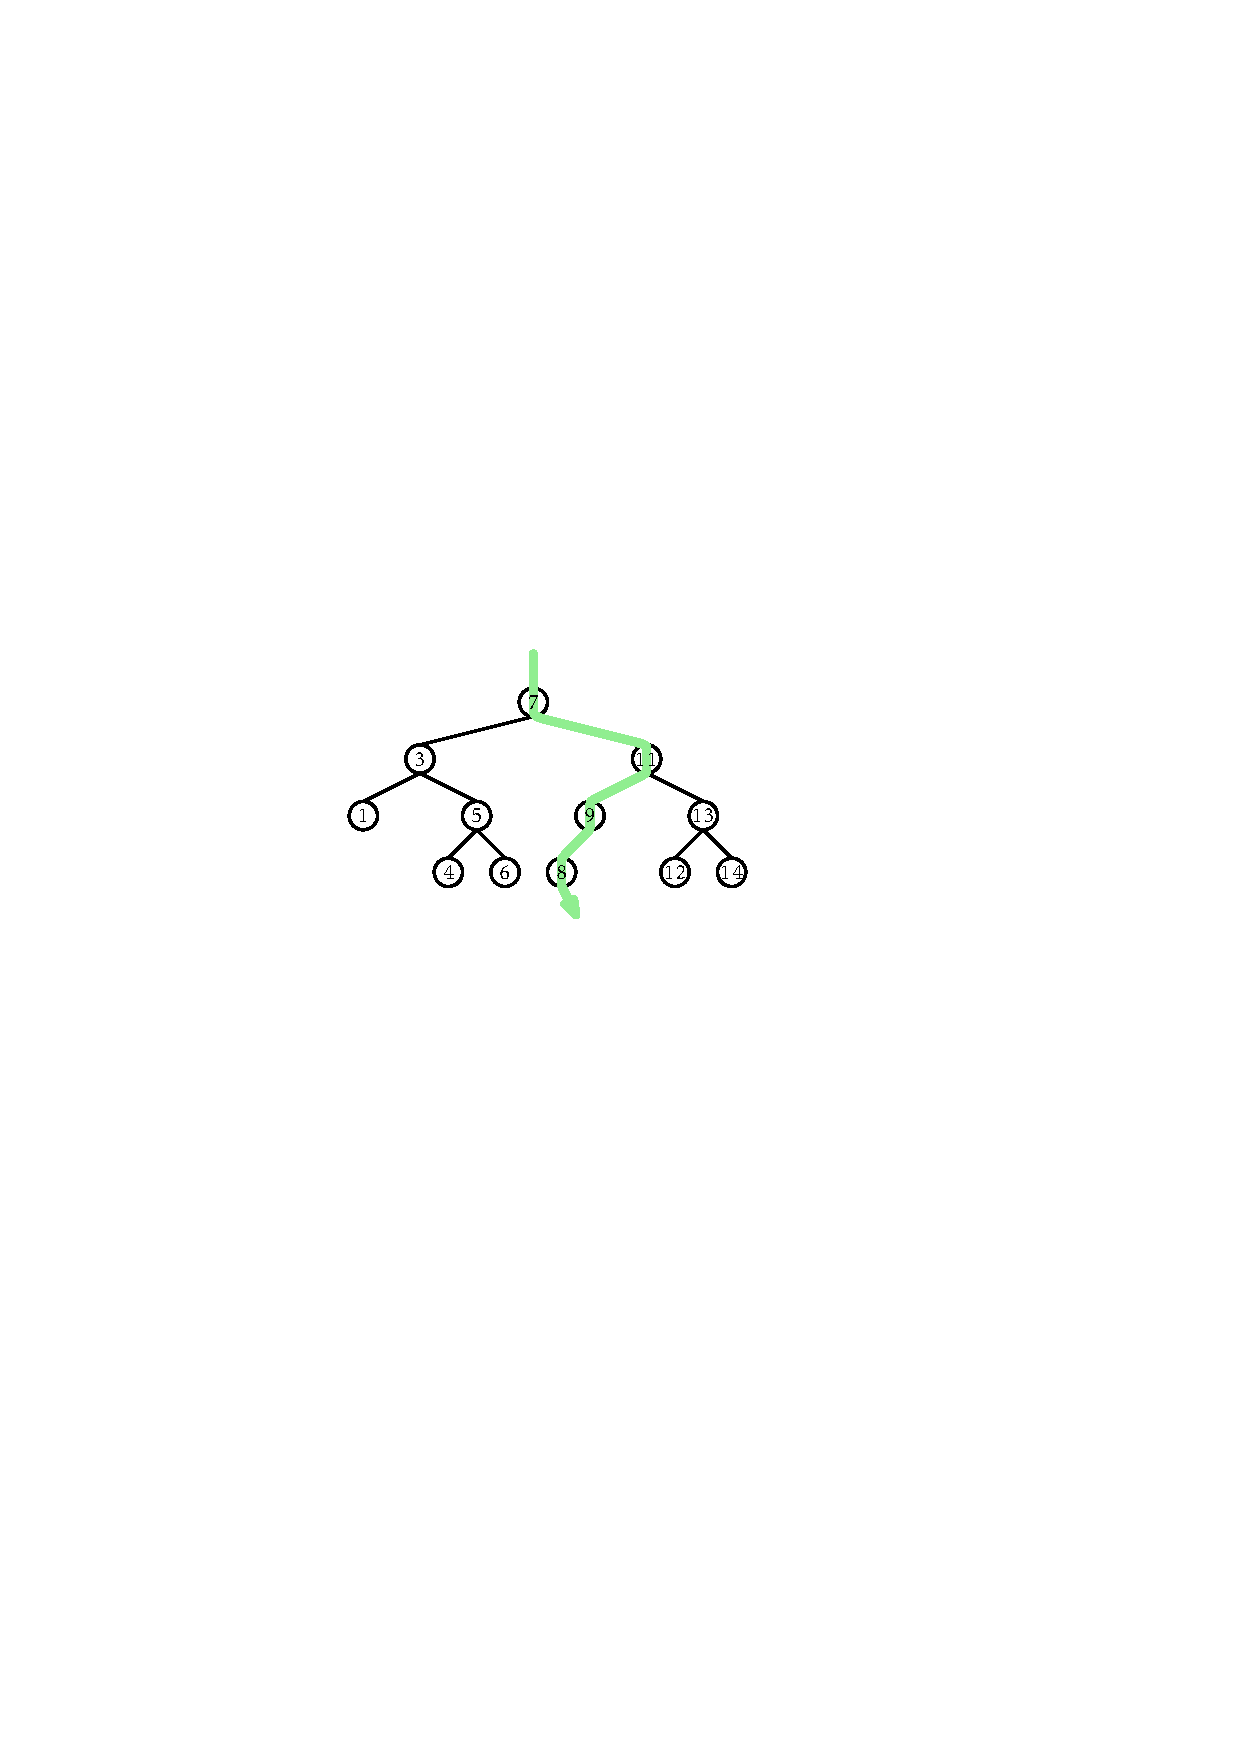
\includegraphics[width=\HalfScaleIfNeeded]{figs/bst-example-4} &
    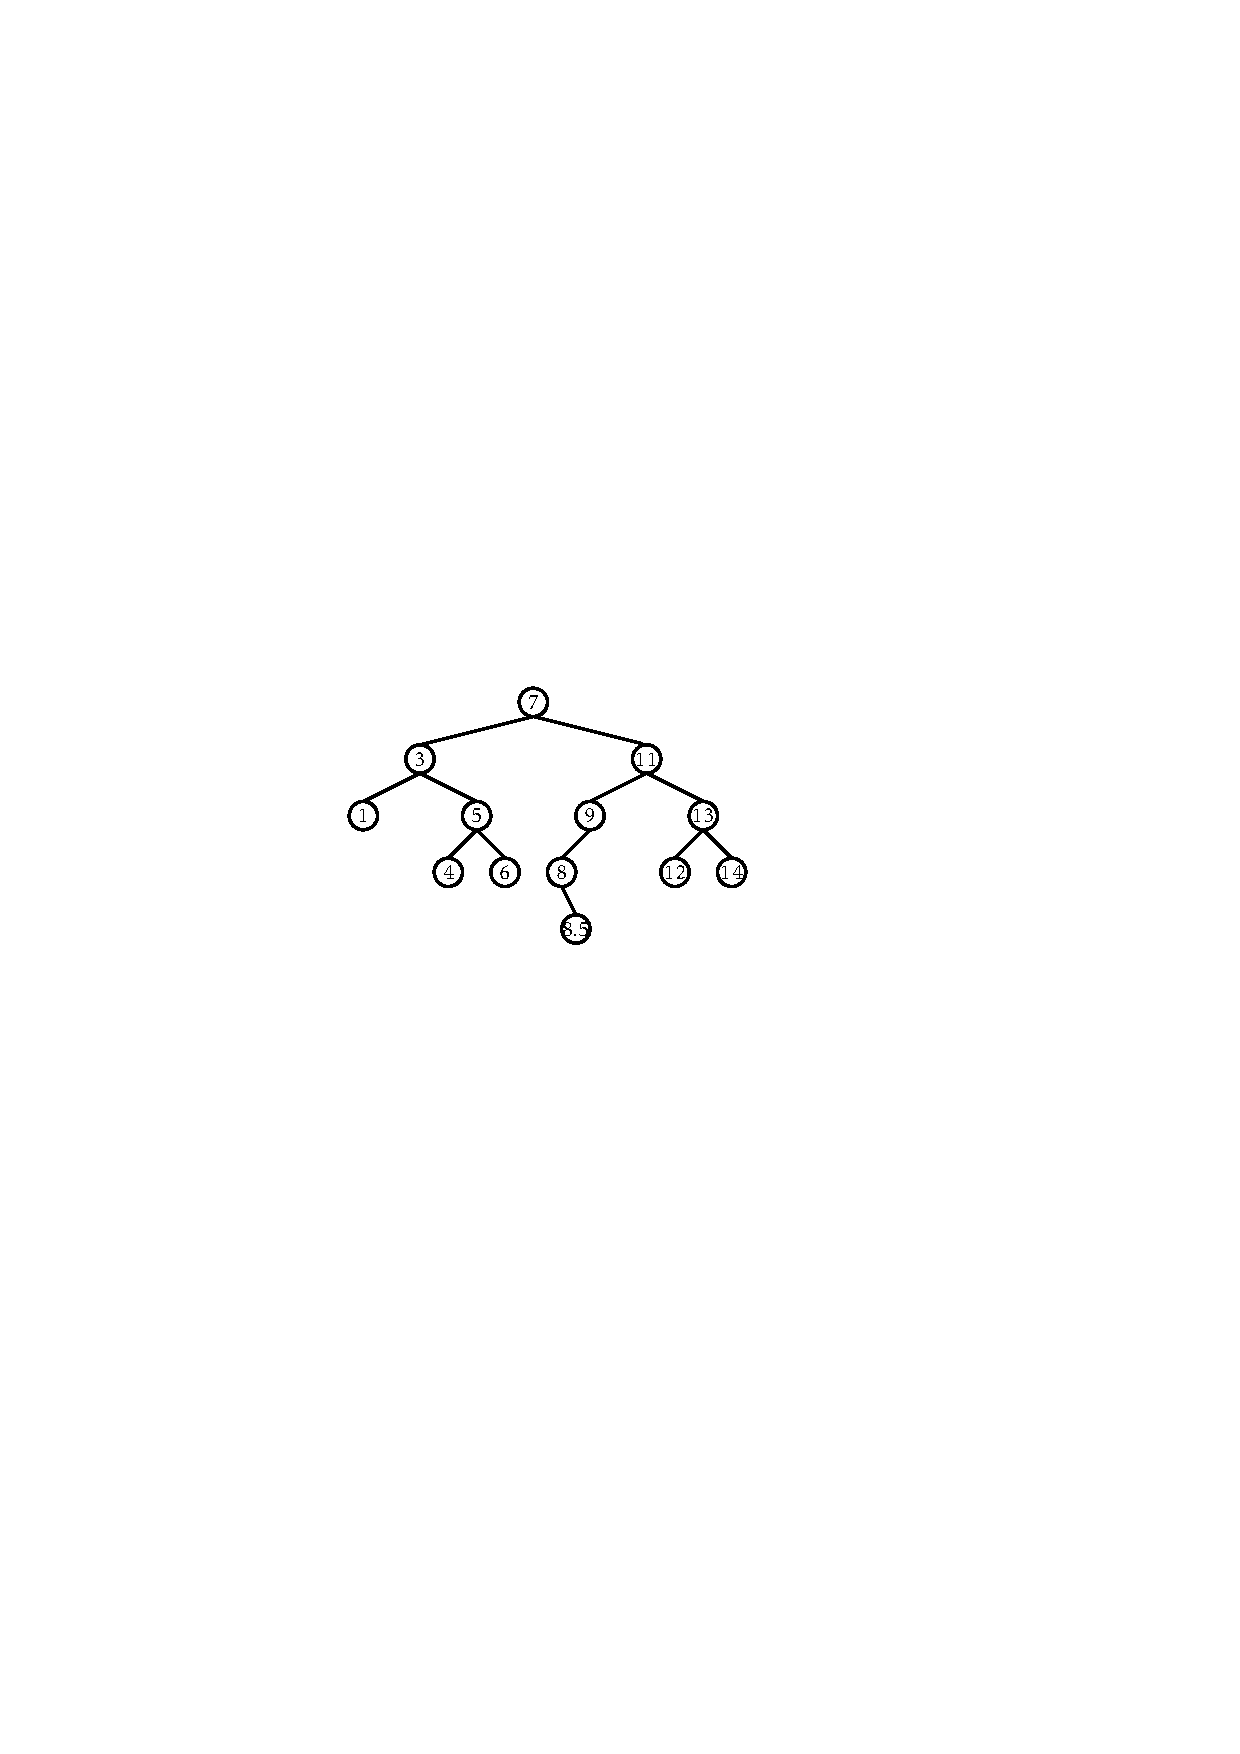
\includegraphics[width=\HalfScaleIfNeeded]{figs/bst-example-5} 
    \end{tabular}
  \end{center}
  \caption{Inderindo o valor $8.5$ na árvore binária de busca.}
  \figlabel{bst-insert}
\end{figure}


\subsection{Remoção}

Apagar um valor armazenado em um nó, #u#, de uma #ArvoreBinariaDeBusca# é um pouco mais difícil.  Se #u# é uma folha, então podemos simplesmente desligar #u# do seu pai.  Melhor ainda: se #u# possui somente um filho, nós podemos separar #u# da árvore fazendo #u.pai# adotar o filho de #u# (veja
\figref{bst-splice}):
\codeimport{ods/BinarySearchTree.splice(u)}

\begin{figure}
  \begin{center}
    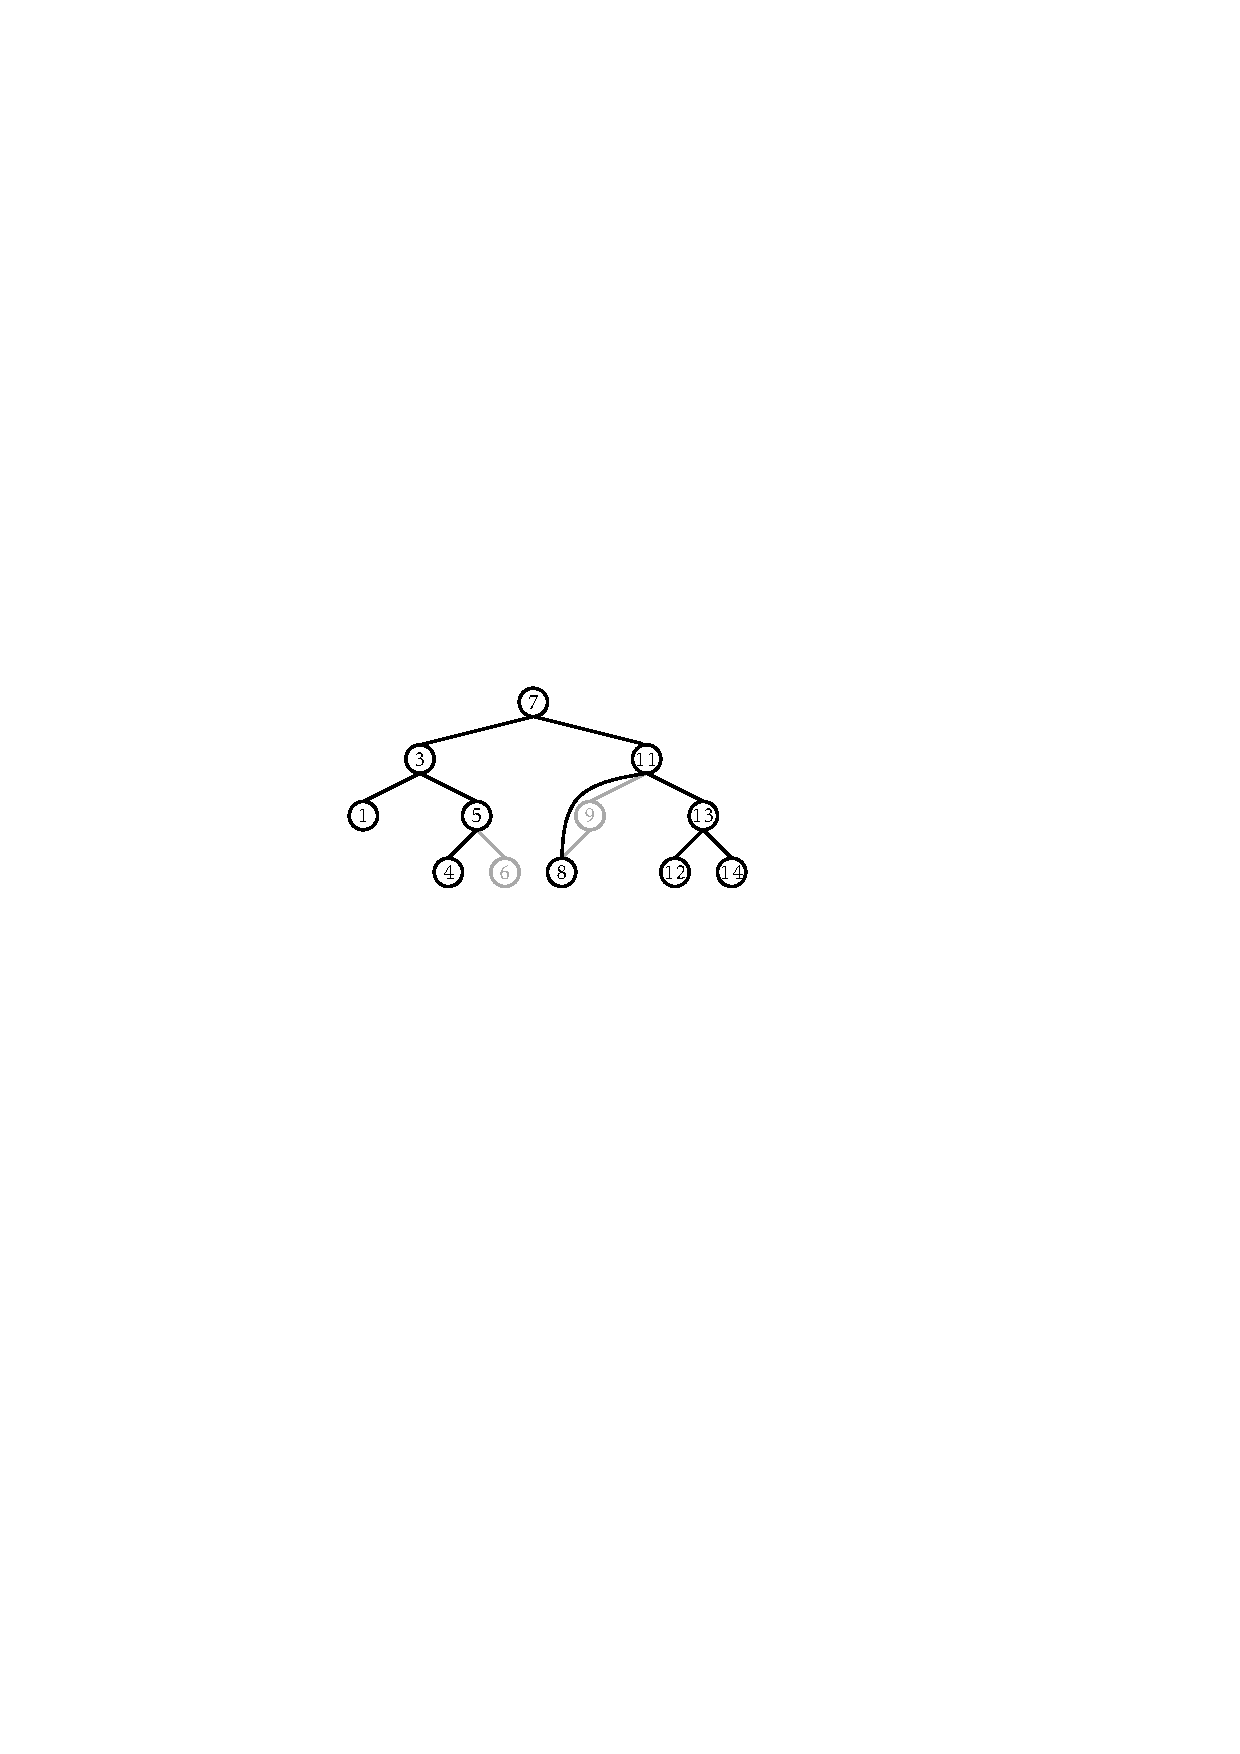
\includegraphics[scale=0.90909]{figs/bst-splice}
  \end{center}
  \caption{Removendo uma folha ($6$) ou um nó com apenas um filho ($9$) é fácil.}
  \figlabel{bst-splice}
\end{figure}

As coisas ficam complicadas, contudo, quando #u# possui dois filhos. Neste caso, a coisa mais simples a fazer é encontrar um nó, #w#, que possua menos que dois filhos de modo que #w.x# possa substituir #u.x#.  Para manter a propriedade da árvore binária de busca, o valor #w.x# deveria ser próximo ao valor de #u.x#.  Por exemplo, escolher #w# tal que #w.x# seja o menor valor maior que #u.x# irá funcionar perfeitamente.  Encontrar o nó #w# é fácil; ele é o menor valor na subárvore com raiz em #u.direito#.  Este nó pode ser removido facilmente porque ele não possui filho esquerdo (veja \figref{bst-remove}).
\javaimport{ods/BinarySearchTree.remove(u)}
\cppimport{ods/BinarySearchTree.remove(u)}
\pcodeimport{ods/BinarySearchTree.remove_node(u)}

\begin{figure}
  \begin{center}
    \begin{tabular}{cc}
    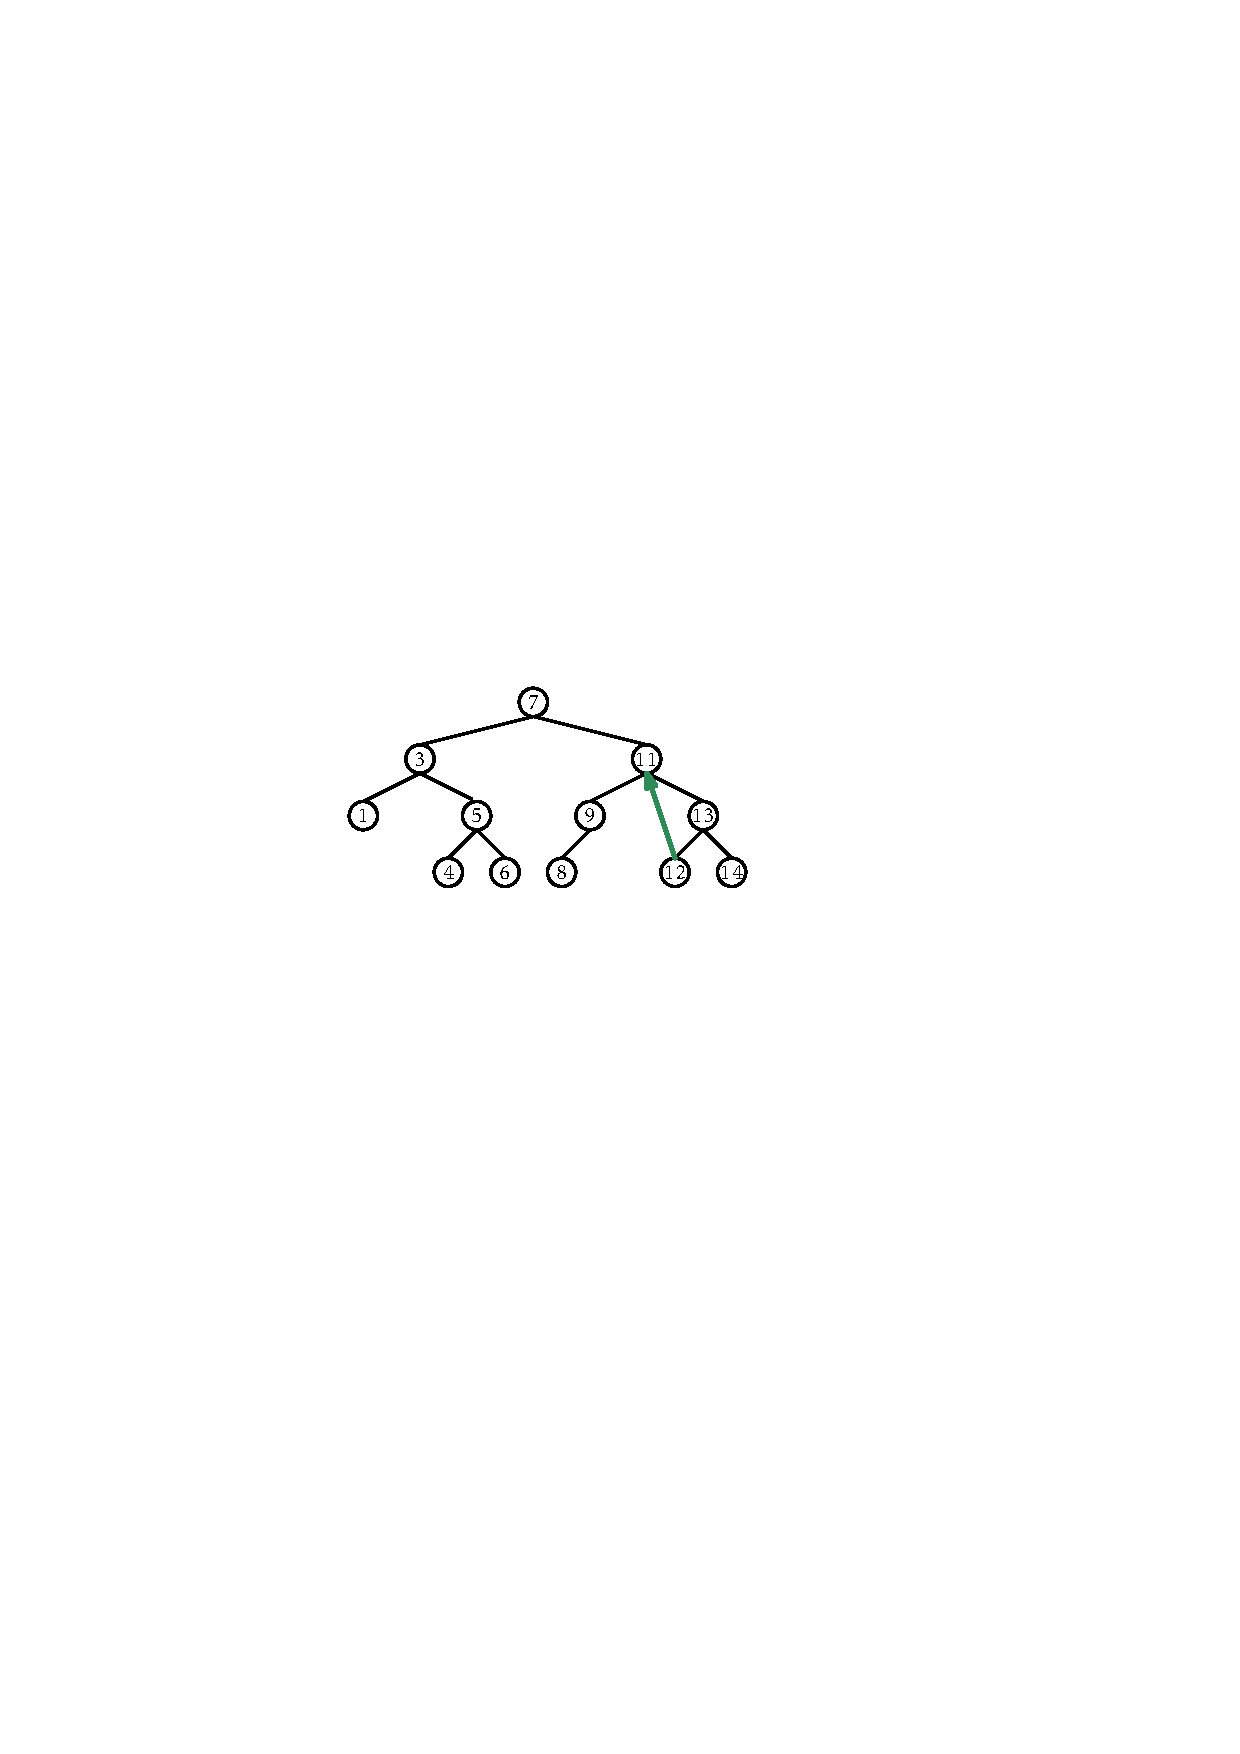
\includegraphics[width=\HalfScaleIfNeeded]{figs/bst-delete-1}
    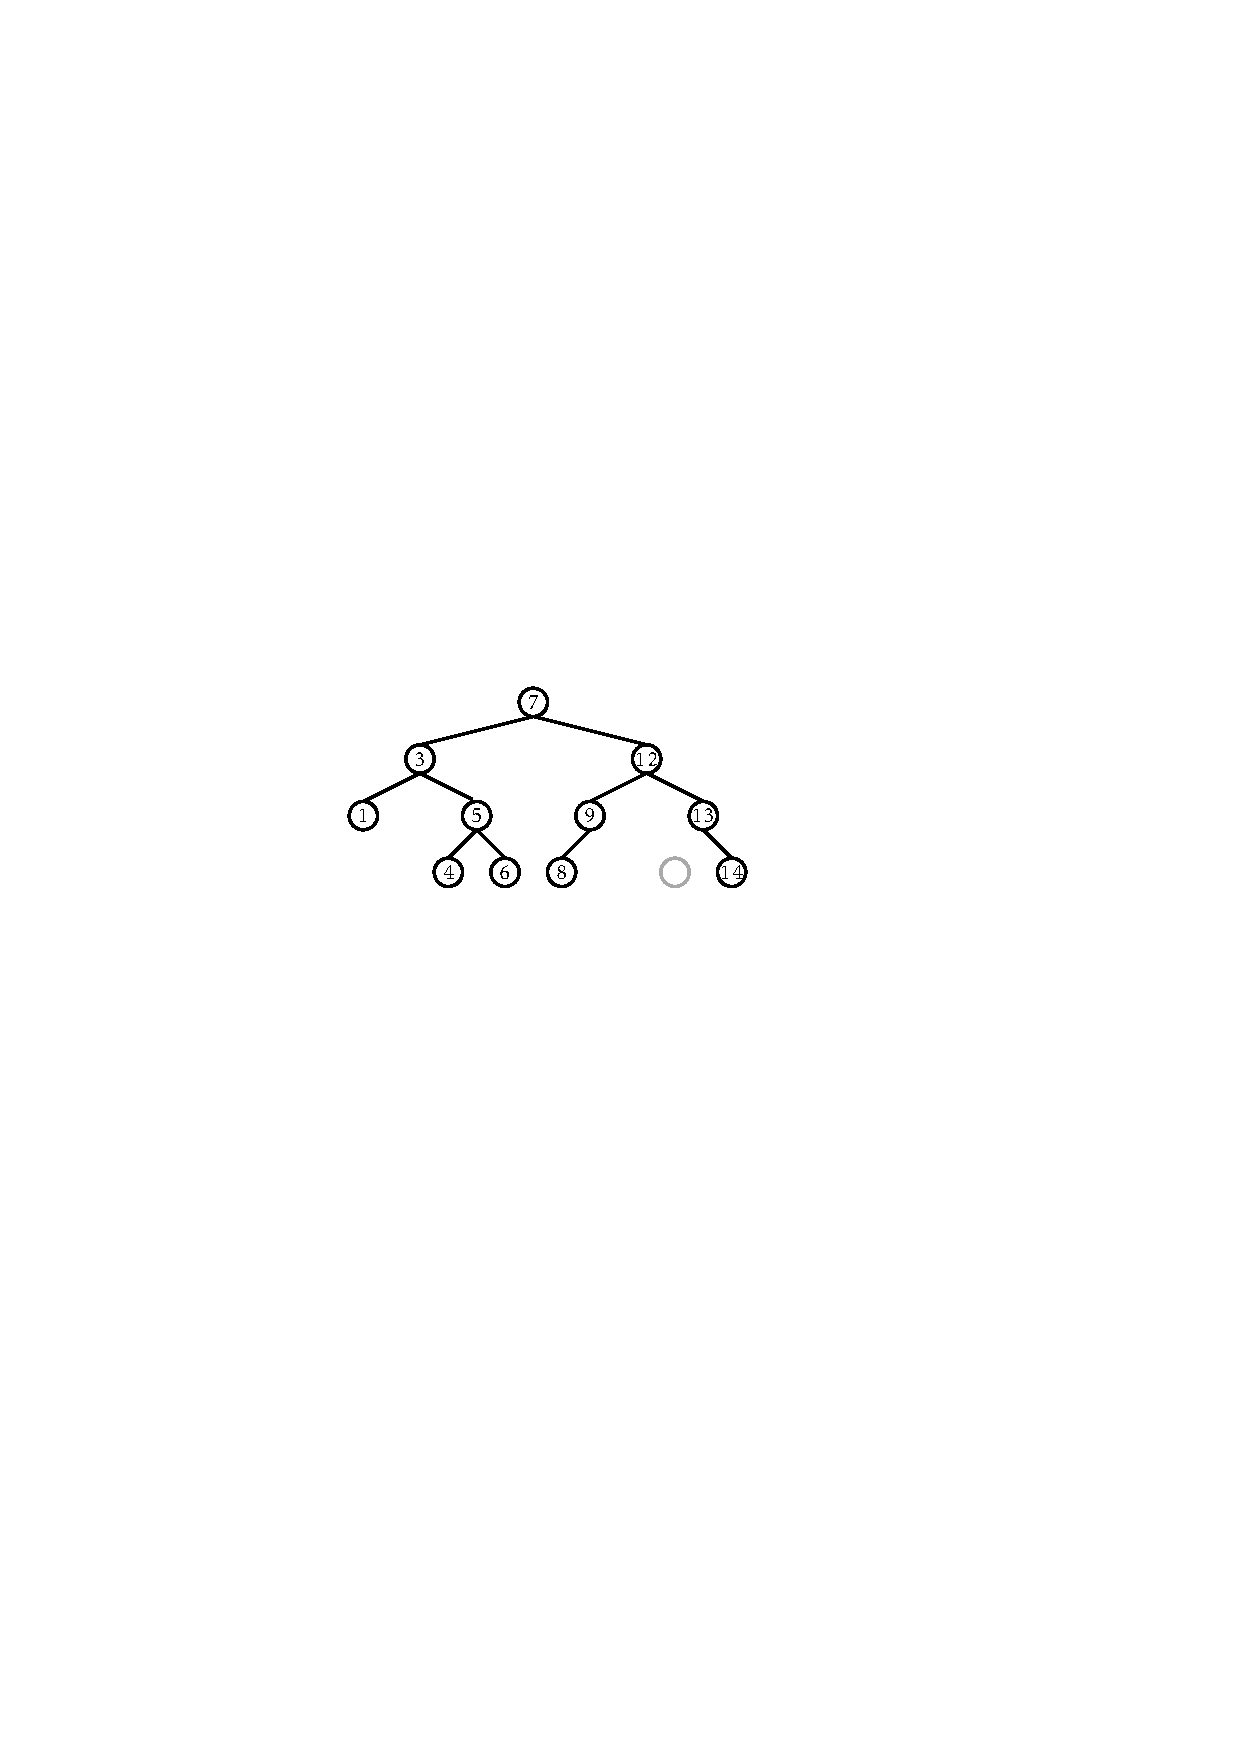
\includegraphics[width=\HalfScaleIfNeeded]{figs/bst-delete-2}
    \end{tabular}
  \end{center}
  \caption[Apagar de uma ArvoreBinariaDeBusca]{Apagar um valor ($11$) de um nó, #u#, com dois filhos é realizado substituindo o valor de #u# pelo menor valor na subárvore direita de #u#.}
  \figlabel{bst-remove}
\end{figure}

\subsection{Resumo}

Cada uma das operações #encontrar(x)#, #inserir(x)#, e #remover(x)# em uma
#ArvoreBinariaDeBusca# envolve seguir um caminho da raiz da árvore até algum nó árvore. Sem conhecer mais sobre o formato da árvore é difícil dizer muito mais sobre o comprimento deste caminho, exceto que ele é menor que #n#, o número de nós na árvore.
O teorema seguinte (não impressionante) resume o desempenho de uma estrutura de dados #ArvoreBinariaDeBusca#:

\begin{thm}\thmlabel{bst}
  #ArvoreBinariaDeBusca# implementa a interface #ConjuntoOrdenado# e suporta as operações #inserir(x)#, #remover(x)#,
  e #encontrar(x)# em $O(#n#)$ tempos por operação.
\end{thm}

\thmref{bst} se compara de modo inferior com o \thmref{skiplist}, que mostra que a estrutura #SkiplistConjuntoOrdenado# pode implementar a interface #ConjuntoOrdenado# com tempo esperado de $O(\log #n#)$ por operação.  O problema com a estrutura da #ArvoreBinariaDeBusca# é que ela pode ficar  \emph{desbalanceada}.
Em vez de parecer como a árvore na \figref{bst} ela pode parecer uma longa sequência de #n# nós, com todos, exceto o último nó possuindo exatamente um único filho.

Existem numerosas formas de evitar uma árvore binária de busca desbalanceada, todos os quais levam a estruturas de dados que têm $O(\log #n#)$ tempos das operações. No \chapref{rbs} mostraremos como tempos de operações \emph{esperados} de $O(\log #n#)$ podem ser atingidos com a aleatoriedade.
No \chapref{scapegoat} mostramos como tempos de operações \emph{amortizados} de $O(\log #n#)$ podem ser alcançados com operações de reconstruções parciais.
No \chapref{redblack} mostramos como tempos de operações de \emph{pior caso} de $O(\log #n#)$ podem ser alcançados com uma árvore que não seja binária: uma nos quais os nós podem ter até quatro filhos.

\section{Discussão e Exercícios}

Árvores Binárias vêm sendo usadas para modelar relacionamentos por milhares de anos. Uma razão para isso é que árvores binárias modelam naturalmente árvores de famílias (pedigree).
\index{árvore de família}%
\index{árvore de família pedigree}%
Essas são as árvores nas quais a raiz é uma pessoa, os filhos esquerdo e direito são os pais da pessoa, e assim sucessivamente, recursivamente.  Nos séculos mais recentes árvore binárias têm também sido usadas para modelar árvores de espécie
\index{árvore de espécies} na biologia, nas quais as folhas da árvore
representam espécies existentes e os nós internos representam
\emph{eventos de especiação}
\index{evento de especiação} nos quais duas populações de uma única espécie evoluem em duas espécies separadas.

Árvores Binárias de Busca parecem ter sido descobertas independentemente por vários grupos nos anos 1950 \cite[Section~6.2.2]{k97v3}.  Referências adicionais para tipos específicos de árvores binárias de busca são fornecidas nos capítulos subsequentes.

Quando implementamos uma árvore binária a partir do zero, várias decisões de projeto devem ser tomadas.  Uma delas é a questão se cada nó guarda um ponteiro para seu pai ou não.  Se a maioria das operações envolvem simplesmente um caminho seguindo da raiz para uma folha, então o ponteiro para o pai é desnecessário, uma perda de espaço e uma fonte potencial de erros de codificação. Por outro lado, a falta do ponteiro para o pai significa que o percurso da árvore deve ser feito recursivamente ou com o uso de uma pilha explícita.  Alguns outros métodos (como inserir ou apagar em alguns tipos de árvores binárias de busca desbalanceadas) são também mais complicados pela ausência do ponteiro para o pai.

Outra decisão de projeto está relacionada em como armazenar o pai, os filhos esquerdo e direito em um nó.  Na implementação fornecida aqui, esses ponteiros são armazenados como variáveis separadas.   Outra opção é armazená-los em um vetor, #p#, de tamanho 3, de modo que #u.p[0]# é o filho esquerdo de #u#, #u.p[1]# é o filho direito de #u#, e #u.p[2]# é o pai de #u#.  O uso do vetor assim implica que algumas sequências do comando #if# podem ser simplificadas em expressões algébricas.

Um exemplo de tal simplificação ocorre durante o percurso na árvore. Se um percurso chega a um nó #u# por #u.p[i]#, então o próximo nó neste percurso é $#u.p#[(#i#+1)\bmod 3]$.  Exemplos similares ocorrem quando existe uma simetria esquerda-direita. Por exemplo, o irmão de #u.p[i]# é $#u.p#[(#i#+1)\bmod 2]$.  Este truque funciona melhor se #u.p[i]# é um filho esquerdo ($#i#=0$) ou um filho direito ($#i#=1$) de #u#.  Em diversos casos isso significa que algum código complicado que de outra maneira precisaria ter ambas versões para os lados esquerdo e direito podem ser escritos apenas uma vez. Veja os métodos #giraEsquerda(u)# and #giraDireita(u)# na página~\pageref{page:rotations}
para um exemplo.

\begin{exc}
  Prove que uma árvore binária com $#n#\ge 1$ nós possui $#n#-1$ arestas.
\end{exc}

\begin{exc}
  Prove que uma árvore binária com $#n#\ge 1$ nós reais (internos) possui $#n#+1$ nós externos.
\end{exc}

\begin{exc}
  Prove que, se uma árvore binária, $T$, possui ao menos uma folha, então ou
  (a)~a raiz de $T$ possui no máximo um filho ou (b)~$T$ possui mais de uma folha.
\end{exc}

\begin{exc}
  Implemente um método não recursivo, #tamanho2(u)#, que calcule o tamanho da subárvore com raiz no nó #u#.
\end{exc}

\begin{exc}
  Escreva um método não recursivo, #altura2(u)#, que calcule a altura do nó #u# em uma #ArvoreBinaria#.
\end{exc}

\begin{exc}
  Uma árvore binária é \emph{balanceada em tamanho}
  \index{balanceada em tamanho}%
  \index{árvore binária de busca!balanceada em tamanho}%
  se, para cada nó #u#, os tamanhos das subárvores com raiz em #u.esquerdo# e #u.direito# diferem de no máximo um.
  Escreva um método recursivo, #ehBalanceada()#, que testa se uma árvore binária é balanceada.  Seu método deve executar num tempo $O(#n#)$.  (Certifique-se de testar seu código  em algumas árvores grandes com diferentes formas; é fácil escrever um método que leve muito mais que $O(#n#)$ em tempo de execução.)
\end{exc}

\index{percurso!pré-ordem}%
\index{percurso!pós-ordem}%
\index{percurso!em-ordem}%
\index{percurso pré-ordem}%
\index{percurso pós-ordem}%
\index{percurso em-ordem}%
Um percurso em \emph{pré-ordem}  de uma árvore binária é um percurso que visita cada nó, #u#, antes de qualquer de seus filhos.  Um percurso \emph{em-ordem} 
visita #u# após ter visitado todos os nós na subárvore esquerda de #u# porém antes de visitar qualquer um dos nós da subárvore direita de #u#.  Um percurso em \emph{pós-ordem} visita #u# somente após ter visitado todos os outros nós nas subárvores de #u#.
A numeração em pré/em/pós-ordem rotula os nós da árvore com inteiros $0,\ldots,#n#-1$ na ordem na qual eles são encontrados por um percurso  pré/em/pós-ordem.  Veja \figref{binarytree-numbering}
para um exemplo.

\begin{figure}
  \begin{center}
    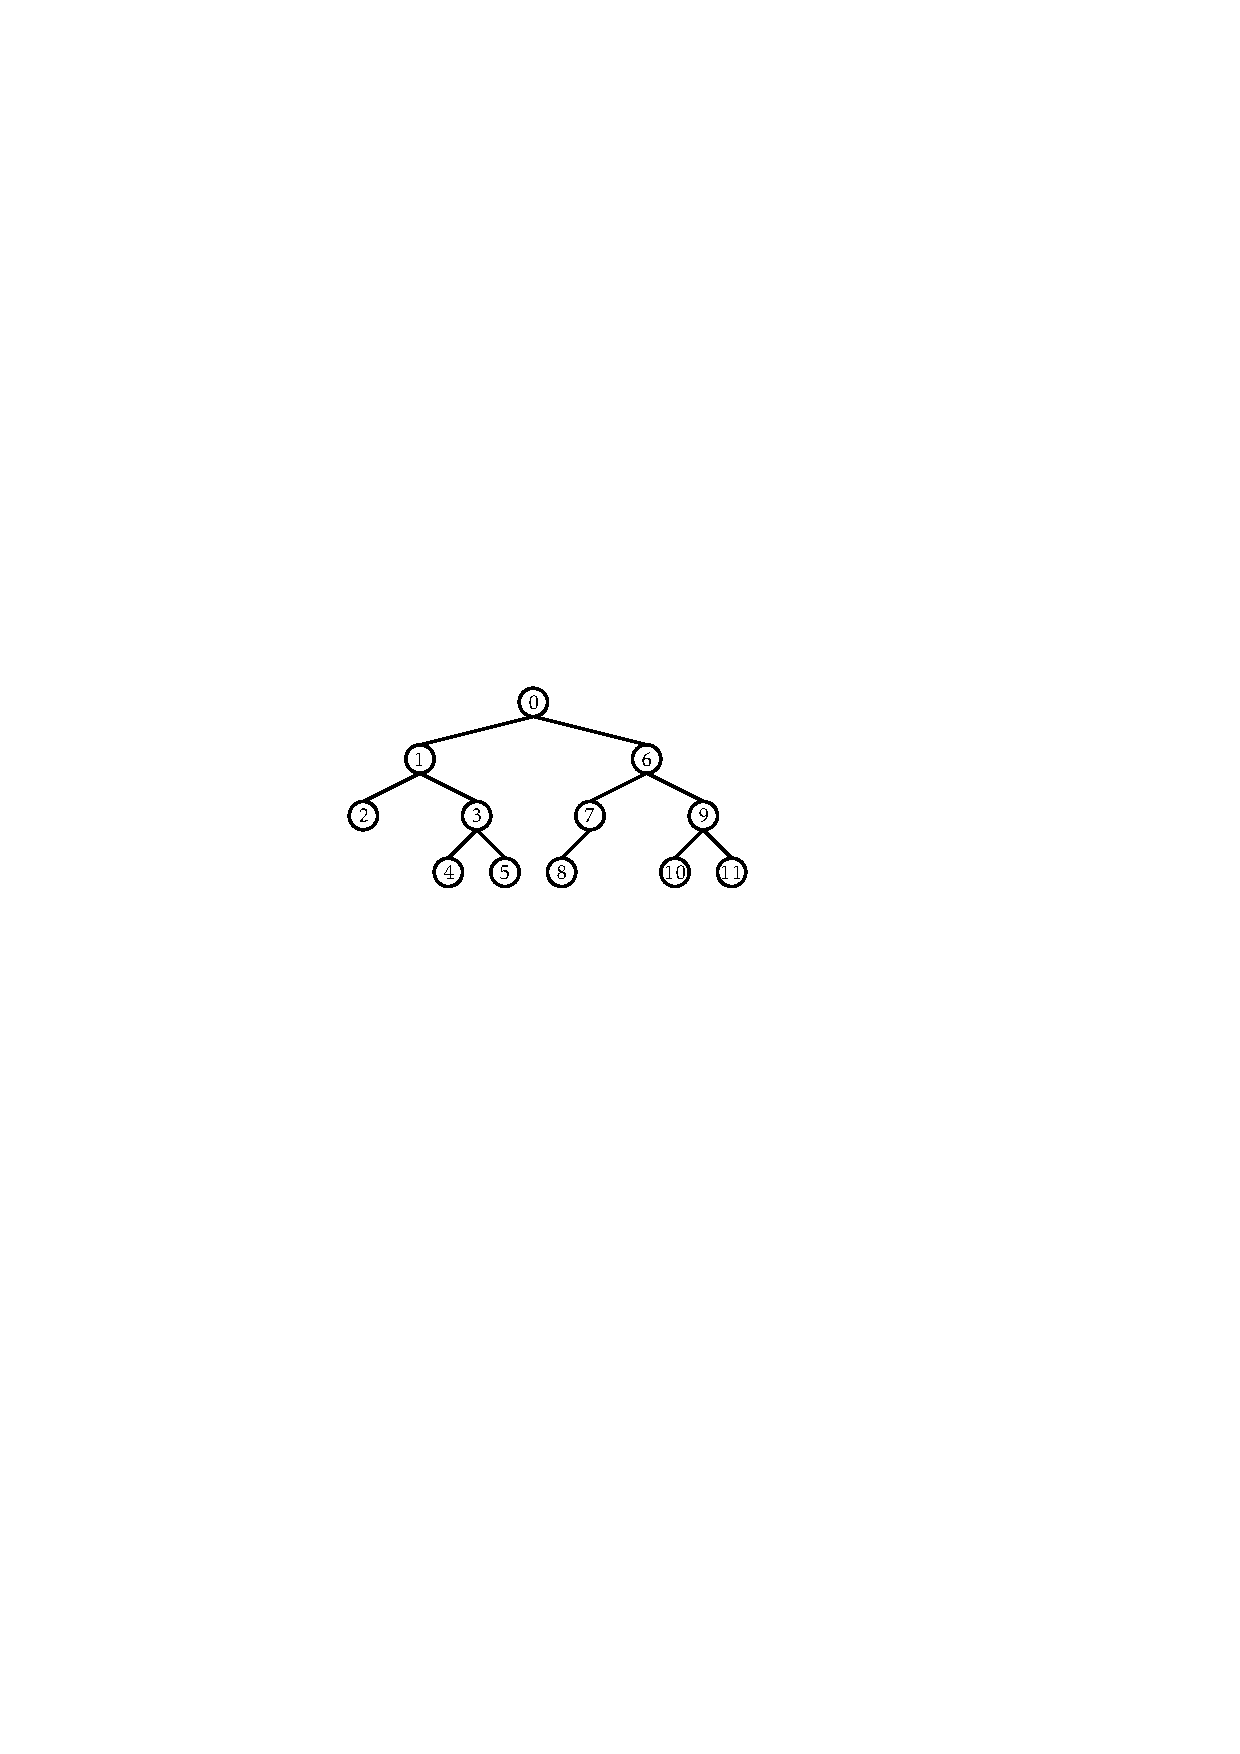
\includegraphics[scale=0.90909]{figs/binarytree-numbering-1}
    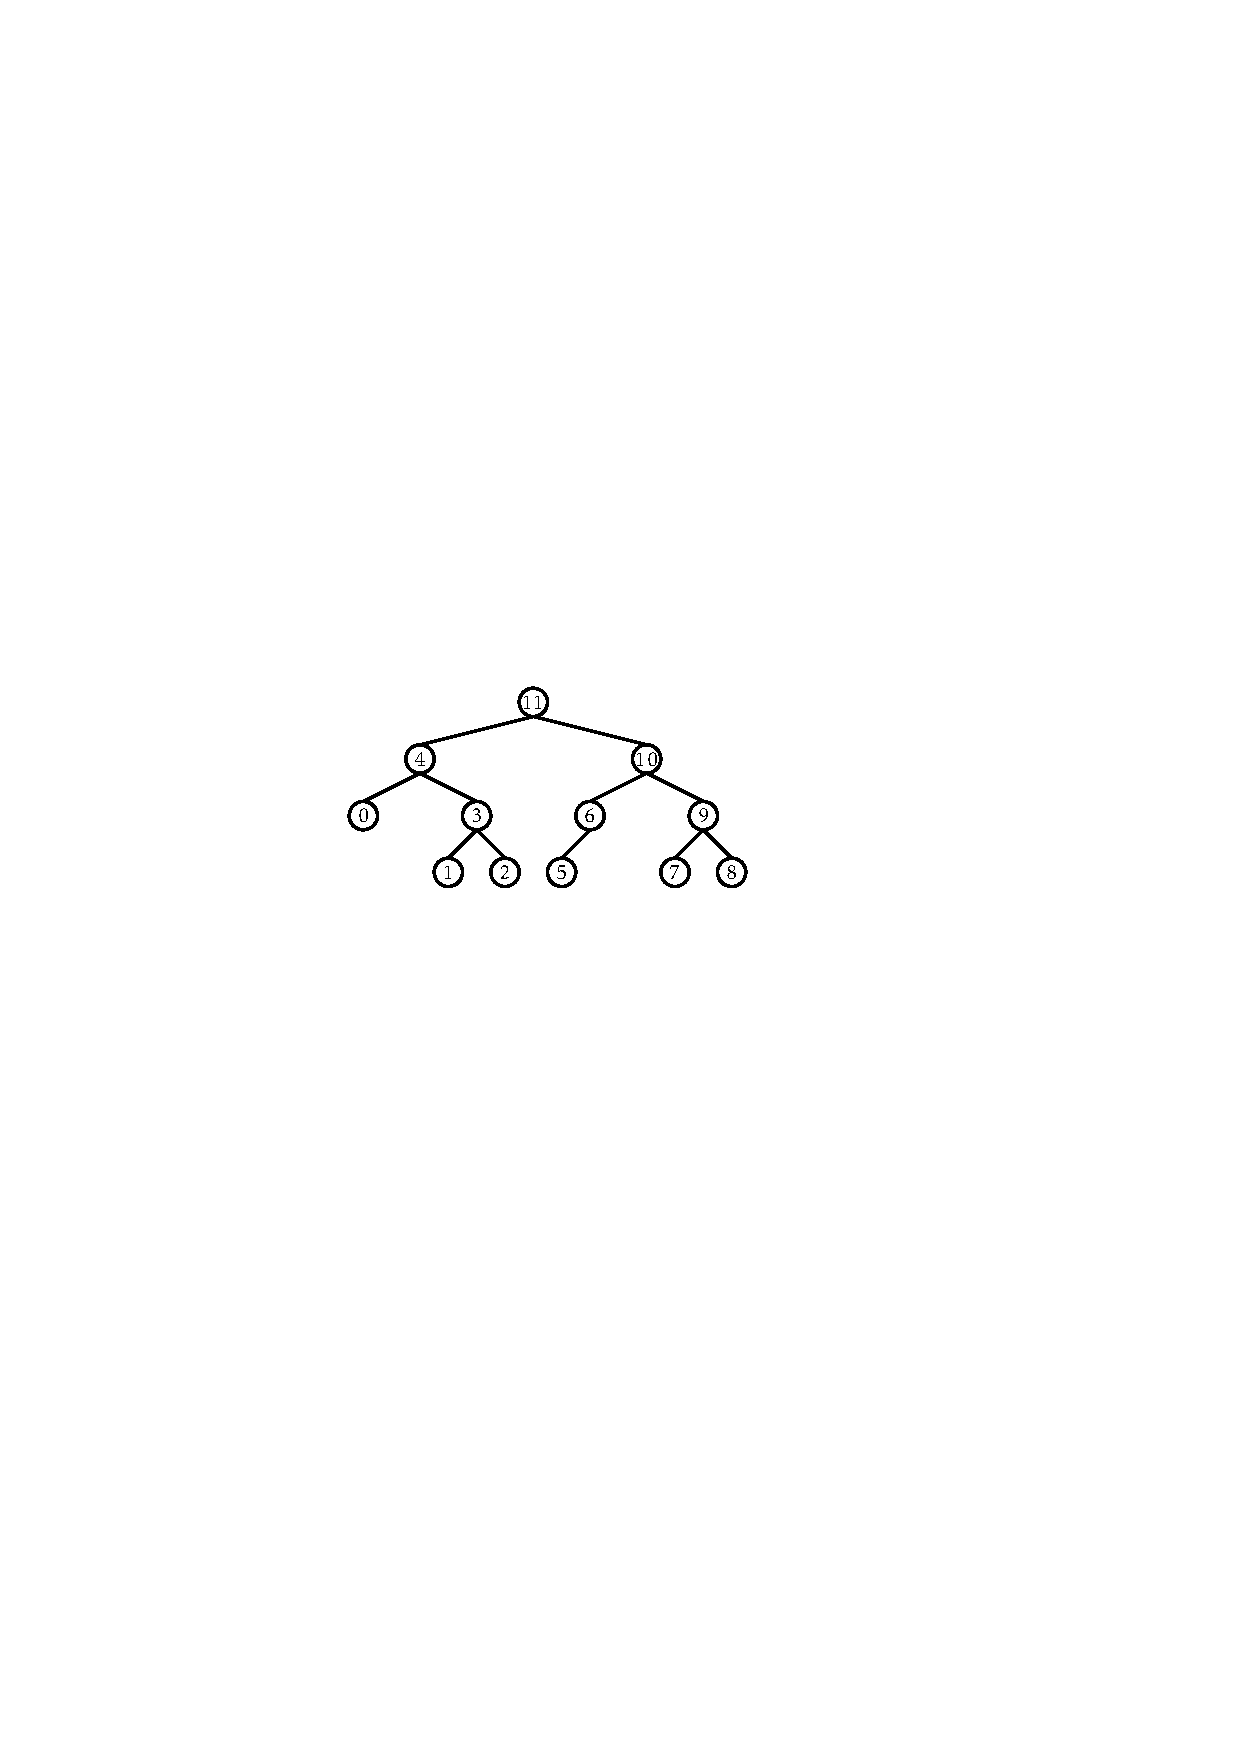
\includegraphics[scale=0.90909]{figs/binarytree-numbering-2} \\[2ex]
    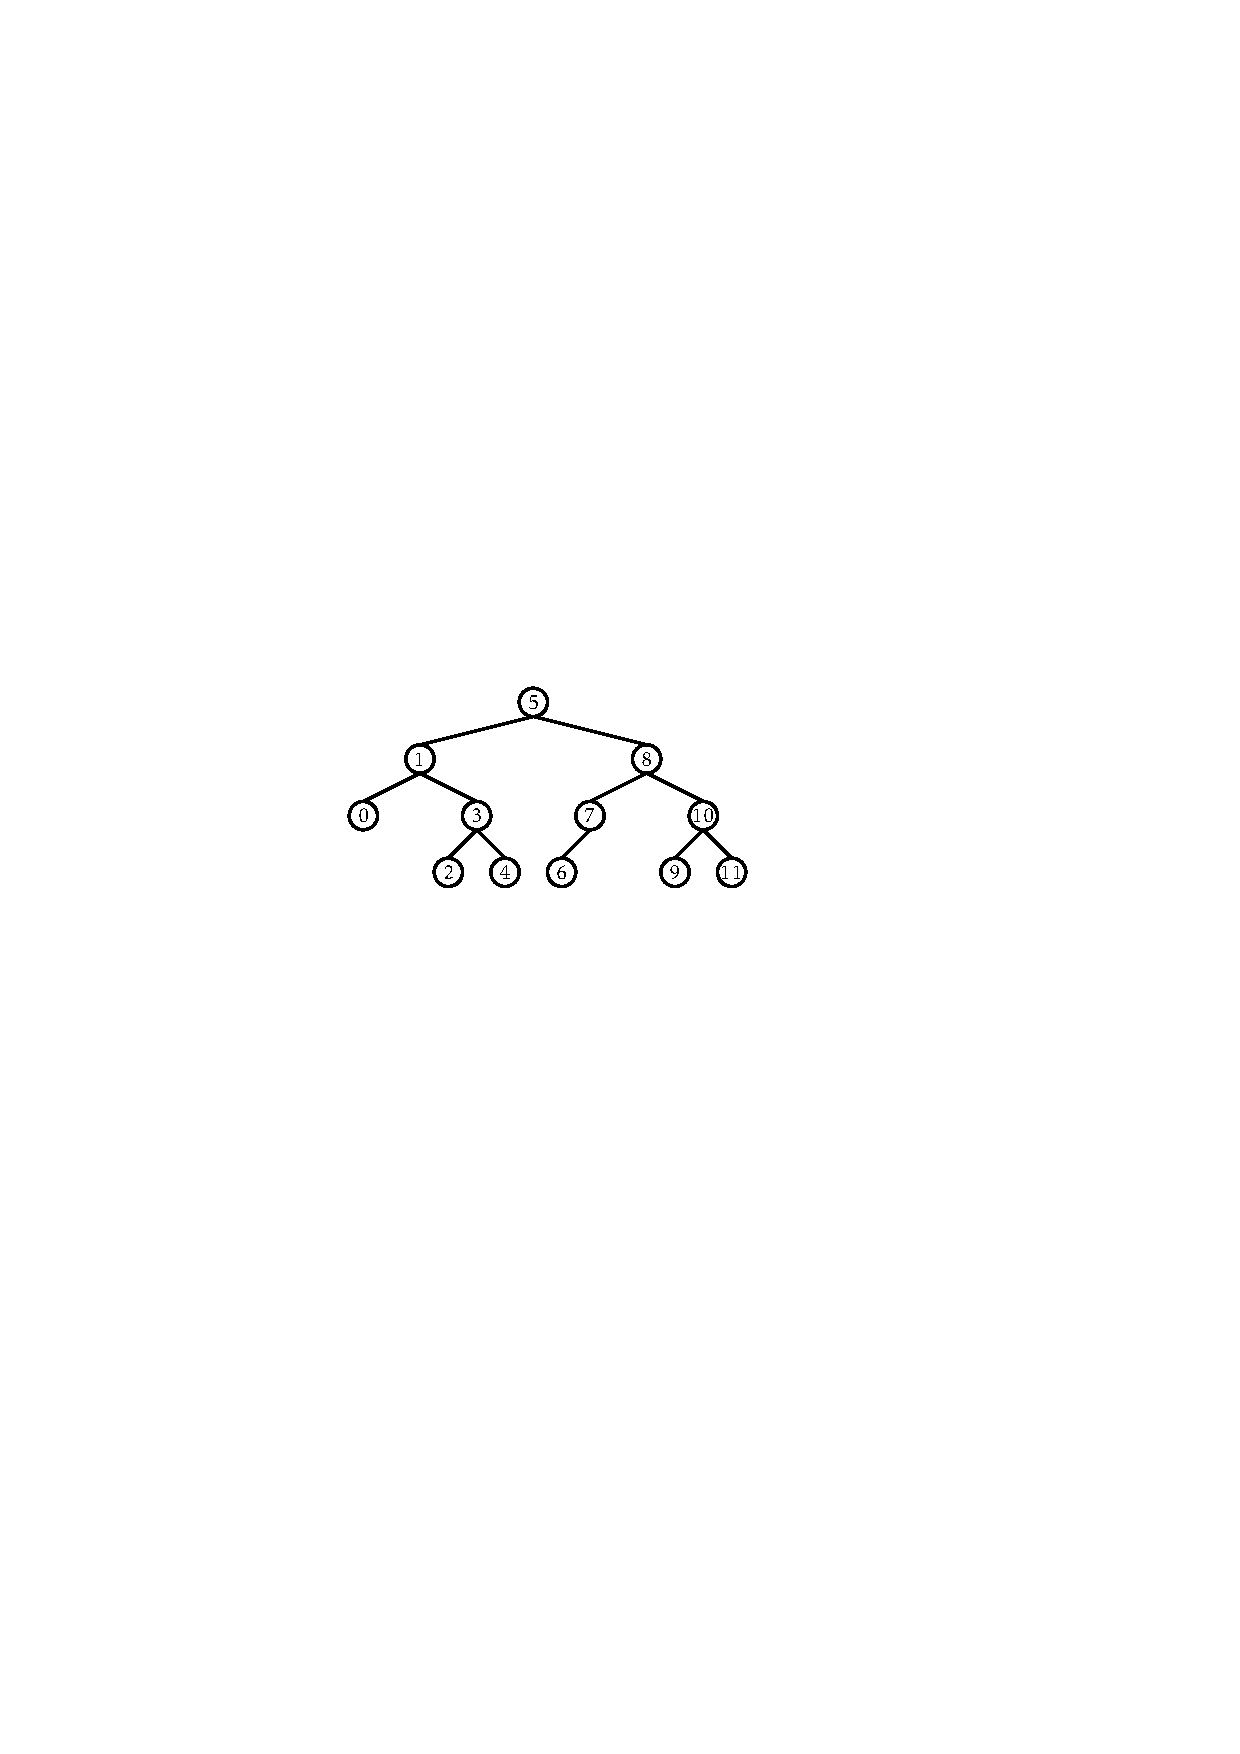
\includegraphics[scale=0.90909]{figs/binarytree-numbering-3}
  \end{center}
  \caption{numeração em pré-ordem, pós-ordem, e em-ordem de uma árvore binária.}
  \figlabel{binarytree-numbering}
\end{figure}

\begin{exc}
  \index{número!pré-ordem}%
  \index{número!pós-ordem}%
  \index{número!em-ordem}%
  \index{número de pré-ordem }%
  \index{número de pós-ordem}%
  \index{número de em-ordem}%
  Crie uma subclasse de #ArvoreBinaria# cujos nós tenham campos para armazenar números de pré-ordem, pós-ordem, e em-ordem.  Escreva os métodos recursivos #numeroPreOrdem()#, #numeroEmOrdem()#, e #numeroPosOrdem()# que atribua esses números corretamente. Esses métodos devem executar num tempo $O(#n#)$.
\end{exc}

\begin{exc}\exclabel{tree-traversal}
  Implemente as funções não recursivas #proxPreOrdem(u)#, #proxEmOrdem(u)#, e #proxPosOrdem(u)# que retornam o nó seguinte a #u# em um percurso em pré-ordem,
  em-ordem, ou pós-ordem, respectivamente.   Essas funções devem ter um tempo de execução amortizado constante; se começamos em qualquer nó
  #u# e repetidamente chamarmos uma dessas funções e atribuirmos o valor retornado a #u# até que $#u#=#null#$, então o custo de todas essas chamadas deveria ser de $O(#n#)$.
\end{exc}

\begin{exc}
  Suponha que temos uma árvore binária com números de pré-, pós-, e em-ordem atribuídos aos nós.  Mostre como esses números podem ser usados para responder cada uma das seguintes questões em tempo constante:
  \begin{enumerate}
    \item Dado um nó #u#, determine o tamanho da subárvore com raiz em #u#.
    \item Dado um nó #u#, determine a profundidade de #u#.
    \item Dados dois nós #u# e #w#, determine se #u# é um ancestral de #w#
  \end{enumerate}
\end{exc}

\begin{exc}
  Suponha que você receba uma lista de nós com números de pré-ordem e em-ordem atribuídos a eles.  Prove que existe no máximo uma possível árvore com esses números de pré-ordem/em-ordem e mostre como construi-la.
\end{exc}

\begin{exc}
  Mostre que o formato de qualquer árvore binária com #n# nós pode ser representada usando no máximo $2(#n#-1)$ bits.  (Dica: pense sobre gravar o que acontece durante o percurso e então recuperar este registro para reconstruir a árvore.)
\end{exc}

\begin{exc}
  Ilustre o que acontece quando adicionamos o valor $3.5$ e depois 4.5 na árvore binária de busca na \figref{bst}.
\end{exc}

\begin{exc}
  Ilustre o que acontece quando removemos o valor $3$ e depois 5 da árvore binária de busca na \figref{bst}.
\end{exc}

\begin{exc}
  Implemente um método para a #ArvoreBinariaDeBusca#, #obtemLE(x)#,
  que retorne uma lista de todos os itens em uma árvore que sejam menores que ou iguais a #x#.  O tempo de execução do seu método deve ser $O(#n#'+#h#)$ no qual $#n#'$ é o número de itens menores que ou iguais a #x# e #h# é a altura da árvore.
\end{exc}

\begin{exc}
  Descreva como inserir os elementos $\{1,\ldots,#n#\}$ para uma  #ArvoreBinariaDeBusca# inicialmente vazia de modo que a árvore resultante tenha altura $#n#-1$.  De quantos modos podemos fazer isso?
\end{exc}

\begin{exc}
  Se temos uma #ArvoreBinariaDeBusca# e executamos a operação #inserir(x)# seguida por #remover(x)# (com o mesmo valor de #x#) necessariamente retornamos à árvore original?
\end{exc}

\begin{exc}
  Uma operação #remover(x)# pode aumentar a altura de algum nó em uma
  #ArvoreBinariaDeBusca#?  Se sim, de quanto?
\end{exc}

\begin{exc}
  Uma operação  #inserir(x)# pode  aumentar a altura de algum nó em uma #ArvoreBinariaDeBusca#?  Se sim, de quanto?
\end{exc}

\begin{exc}
  Projete e implemente uma versão da #ArvoreBinariaDeBusca# na qual cada nó, #u#, mantém os valores #u.tamanho# (o tamanho da subárvore com raiz em #u#), #u.profundidade# (a profundidade de #u#), e #u.altura# (a altura da subárvore com raiz em #u#).  

  Estes valores devem ser mantidos mesmo durante chamadas a operações de #inserir(x)# e #remover(x)#, porém isto não deve aumentar o custo dessas operações de mais de um valor constante.
\end{exc}
